\documentclass{article}

% --- PACKAGES ---
\usepackage[utf8]{inputenc}
\usepackage{amsmath}         % For math environments
\usepackage[margin=1in]{geometry} % Added standard margins
\usepackage{graphicx}        % For images (though none here)
\usepackage{booktabs}        % For professional tables
\usepackage{hyperref}        % For links (though none here)
\usepackage{rotating}   % You already have this
\usepackage{lscape}     % Add this for the landscape environment
\usepackage{longtable}  % Add this for the longtable environment
\usepackage{geometry}
\usepackage{array}
\usepackage{tikz}
\usetikzlibrary{shapes.geometric, arrows.meta, positioning, fit, calc}
\usepackage{listings}
\usepackage{color}
\usepackage{xcolor}

\lstdefinestyle{fortran-iv-style}{
	language=[90]Fortran,        % Use the Fortran driver
	basicstyle=\ttfamily\small,  % Font style and size
	numbers=left,                % Line numbers on the left
	numberstyle=\tiny\color{gray}, % Style of the line numbers
	stepnumber=1,                % Number every line
	numbersep=5pt,               % Distance of line numbers from code
	commentstyle=\color{green!50!black}, % Style of comments
	keywordstyle=\color{red}\bfseries,   % Style of keywords
	stringstyle=\color{purple},          % Style of strings
	showspaces=false,            % Do not underline spaces
	showstringspaces=false,      % Do not underline spaces in strings
	tabsize=4,                   % Set tab size to 4 spaces
	breaklines=true,             % Enable automatic line breaking
	frame=single,                % Add a frame around the listing
	backgroundcolor=\color{gray!10}, % Light gray background
	captionpos=b,                % Caption position at the bottom
	morecomment=[l]{!},          % Treat '!' as a line comment starter (Fortran 90 standard, but widely used)
}

\lstset{style=fortran-iv-style}




% --- DOCUMENT INFO ---
\title{ANALYTICAL STUDY OF CATALYTIC REACTORS FOR HYDRAZINE DECOMPOSITION: \\
	ONE-AND TWO-DIMENSIONAL STEADY-STATE PROGRAMS}
\author{E.J. SMITH, D.B. SMITH and A.S. KESTEN}
\date{AUGUST, 1968}

% --- BEGIN DOCUMENT ---
\begin{document}
	
	\maketitle
	
	\begin{center}
		Prepared for \\
		NATIONAL AERONAUTICS AND SPACE ADMINISTRATION \\
		CONTRACT NAS 7-458 \\
		\vspace{1em}
		United Aircraft Research Laboratories \\
		UNITED AIRCRAFT CORPORATION
	\end{center}
	
	\newpage
	
	% --- ABSTRACT ---
	\begin{abstract}
		Two machine computational programs have been developed under NASA Contract 7-458 to calculate the steady-state temperature and reactant concentration distributions in typical catalyzed hydrazine decomposition reaction chambers.
		One program is based upon a one-dimensional model of the reactor system which describes the behavior of reactors having radially uniform injection profiles and catalyst bed configurations, while the other program is based upon a two-dimensional model which permits consideration of nonuniform radial injection and of catalyst bed configurations exhibiting both radial and axial nonuniformities.
		The one and two-dimensional models and the computer programs developed from these models are described in detail in this computer manual.
		The manual contains operating instructions for these programs as well as descriptions of input and output formats.
		Also included is a discussion of possible operations problems which might arise together with appropriate means for solving these problems.
	\end{abstract}
	
	% --- FOREWORD ---
	\section*{Foreword}
	This work was performed by United Aircraft Research Laboratories for the National Aeronautics and Space Administration under Contract NAS 7-458 initiated April 15, 1966.
	
	Included among those who cooperated in performance of the work under NAS 7-458 were Dr. A. S. Kesten, Program Manager, Dr. W. G. Burwell, Chief, Kinetics and Thermal Sciences Section, Mr. D. B. Smith, Project Analyst, and Mrs. E. J. Smith, Applied Mathematician.
	This work was conducted under program management of the NASA Chief, Liquid Propulsion Experimental Engineering Systems, NASA Headquarters, Washington, D. C., and the Technical Manager was Mr. T. W. Price, Jet Propulsion Laboratory, Pasadena, California.
	
	% --- SUMMARY ---
	\section*{Summary}
	A description is contained herein of two machine computational programs developed under Contract NAS 7-458 with the National Aeronautics and Space Administration.
	These programs represent one- and two-dimensional steady-state models of catalyzed hydrazine decomposition reaction chambers.
	Both of these models consider both thermal and catalytic decomposition of reactants, along with simultaneous heat and mass transfer between the free-gas phase and the gas within the pores of the catalyst pellets.
	The one-dimensional model of the reactor system describes the behavior of reactors having radially uniform injection profiles and catalyst bed configurations, while the two-dimensional model permits consideration of nonuniform radial injection and of catalyst bed configurations exhibiting both radial and axial nonuniformities.
	
	A general description of the one and two-dimensional models and a discussion of the machine programs developed from these models are contained in this manual.
	A description of input and output for both the one and two-dimensional steady-state programs are included in the discussion together with examples of typical data cases.
	Also included is a description of several operational problems which might be encountered while using the programs along with appropriate means for solving these problems.
	In addition, a short write-up of the subroutines contained in each deck is included along with general flow charts of the major routines.
	
	% --- INTRODUCTION ---
	\section{Introduction}
	Under Contract NAS 7-458, the Research Laboratories of United Aircraft Corporation are performing analytical studies of the behavior of distributed-feed catalytic reactors for hydrazine decomposition.
	The specific objectives of this program are (a) to develop computer programs for predicting the temperature and concentration distributions in monopropellant hydrazine catalytic reactors in which hydrazine can be injected at arbitrary locations in the reaction chamber and (b) to perform calculations using these computer programs to demonstrate the effects of various system parameters on the performance of the reactor.
	
	Progress previously reported in the first annual report (Ref. 1) included the development of a computer program which describes the steady-state behavior of a continuous flow type reactor system in which complete radial mixing in the free-gas (or liquid) phase was assumed.
	Progress previously reported in the second annual report (Ref. 2) included an extension of the steady-state program to include radial as well as axial variations in temperature and concentrations in order to permit an analysis of various injection schemes and catalyst bed configurations which exhibit radial nonuniformities.
	These programs had been used to calculate temperature and reactant concentration distributions as functions of feed temperature, chamber pressure, mass flow rate distribution, catalyst size distribution, and embedded injector locations.
	As part of the third year of contract effort attention has been directed toward preparing a manual describing to potential users the operation of these computer programs.
	The manual includes a general description of the one and two-dimensional models as well as a detailed discussion of the machine programs representing these models.
	
	% --- DESCRIPTION OF ANALYSES ---
	\section{Description of Analyses}
	The analysis of a hydrazine engine reaction system carried out to date pertains to a reaction chamber of arbitrary cross section packed with catalyst particles into which liquid hydrazine is injected at arbitrarily selected locations.
	Catalyst particles are represented as "equivalent" spheres with a diameter taken as a function of the particle size and shape.
	Both thermal and catalytic vapor phase decomposition of hydrazine and ammonia are considered in developing equations describing the concentration distributions of these reactants.
	Diffusion of reactants from the free-gas phase to the outside surface of the catalyst pellets is taken into account.
	Since the catalyst material is impregnated on the interior and exterior surfaces of porous particles, the diffusion of reactants into the porous structure must also be considered.
	In addition, the conduction of heat within the porous particles must be taken into account since the decomposition reactions are accompanied by the evolution or absorption of heat.
	
	\subsection{One-Dimensional Steady-State Model}
	In developing the one-dimensional steady-state model, the temperature and reactant concentrations in the interstitial phase (i.e., the free-fluid phase as distinguished from the gas phase within the porous particles) are assumed to vary only with axial distance along the bed.
	In the entrance region of the reaction chamber, where the temperature is low enough to permit the existence of liquid hydrazine, vaporization of liquid is assumed to occur as a result of decomposition of vapor hydrazine within the pores of the catalyst particles.
	That is, catalytic reaction is assumed to be fast enough to keep liquid hydrazine from wetting the pores of the particles;
	the hydrazine concentration at the surface of the catalyst particles at any axial location in the entrance region is then computed from the vapor pressure of liquid hydrazine in the interstitial phase at the same axial location.
	Neglecting axial diffusion of heat or mass, the change in enthalpy of the interstitial phase in the region where liquid hydrazine is present (i.e., where $h_{i} \le h_{i}^{V}$) is related to the concentration gradient at the surface of the porous catalyst particles by
	\begin{equation}
		G\frac{dh}{dz} + H^{N_{2}H_{4}}D_{p}A_{p}\left(\frac{dC_{P}^{N_{2}H_{4}}}{dx}\right)_{s} + F(h_{i}-h_{F})=0 \quad \text{for } h_{i} \le h_{i}^{V}
	\end{equation}
	The variation of mass flow rate, G, with axial distance is easily computed from the rate of feed of liquid hydrazine from the distributed injectors into the system.
	In the region where liquid hydrazine exists at temperatures below the vaporization temperature, the temperature may be obtained from
	\begin{equation}
		T_{i}=T_{F}+\frac{h_{i}-h_{F}}{C_{F}} \quad \text{for } h_{i} < h_{i}^{L}
	\end{equation}
	In the two-phase region, where $T_i = T_{vap}$, the weight-fraction of vapor may be computed from
	\begin{equation*}
		\text{WEIGHT FRACTION VAPOR} = \frac{h_{i}-h_{i}^{L}}{h_{i}^{V}-h_{i}^{L}} \quad \text{for } h_{i}^{L} \le h_{i} \le h_{i}^{V}
	\end{equation*}
	At the axial position at which the enthalpy of the interstitial phase is just equal to the enthalpy of vapor hydrazine at the boiling point ($h_{i} = h_{i}^{V}$), the fraction of hydrazine injected upstream of that point which has been decomposed is easily calculated from an overall heat balance.
	The associated amounts of ammonia, nitrogen, and hydrogen formed from decomposition of hydrazine can then be calculated taking the decomposition reaction as
	\begin{equation}
		2N_{2}H_{4} \rightarrow 2NH_{3}+N_{2}+H_{2}
	\end{equation}
	It should be noted that this is the overall reaction scheme determined experimentally for both homogeneous decomposition of hydrazine (Refs. 3, 4, 5) and low pressure heterogeneous decomposition of hydrazine on platinum surfaces (Ref. 6).\footnote{It is more commonly assumed, without benefit of experimental evidence, that the decomposition reaction is $3 N_{2}H_{4} \rightarrow 4 NH_{3}+N_{2}$, followed by dissociation of one of the four ammonia molecules to nitrogen and hydrogen.
		This two-step process leads to the same overall reaction cited above but assumes that a minimum of 25 percent of the ammonia produced by hydrazine decomposition also decomposes.
		The fractional ammonia dissociation, f, calculated assuming the validity of the two-step process is related by the fractional ammonia dissociation calculated in the present report by
		$$ (f)_{\text{two-step process}} = \frac{3}{4} (f)_{\text{present report}} + \frac{1}{4} $$
	}
	
	In the remainder of the reaction camber, where $h_{i} > h_{i}^{V}$, heat is being supplied to the system by homogeneous as well as heterogeneous decomposition of hydrazine.
	In addition, at sufficiently high temperature, heat is removed from the system by the endothermic decomposition of ammonia.
	For $h_{i} > h_{i}^{V}$ then, the change in enthalpy with axial distance is related to the reactant concentrations in the interstitial phase and at the surface of the porous catalyst particles by
	\begin{equation}
		\frac{d h_{i}}{d z}=-\frac{1}{G}\left\{F(h_{i}-h_{F})+A_{p}h_{c}[T_{i}-(T_{p})_{s}]+H^{N_{2}H_{4}}r_{hom}^{N_{2}H_{4}}\delta\right\}
	\end{equation}
	The changes in reactant weight fractions in the interstitial phase with axial distance are related to the reactant concentrations in the interstitial phase and at the surface of the porous catalyst particles by
	\begin{equation}
		\frac{d{w_{i}}^{N_{2}H_{4}}}{d z}=\frac{1}{G}\left\{F-r_{hom}^{N_{2}H_{4}}\delta - A_{p}(k_{c}c_{i})^{N_{2}H_{4}} - F\left(\frac{c_{i}}{\rho_{i}}\right)^{N_{2}H_{4}}\right\}
	\end{equation}
	\begin{equation}
		\begin{split}
			\frac{d{w_{i}}^{NH_{3}}}{dz}=\frac{1}{G}\left\{r_{hom}^{N_{2}H_{4}}\delta\frac{M^{NH_{3}}}{M^{N_{2}H_{4}}}\right. & +A_{p}(k_{c}c_{i})^{N_{2}H_{4}}\frac{M^{NH_{3}}}{M^{N_{2}H_{4}}} \\
			& \left. - A_{P}\left(k_{c}[c_{i}-(c_{p})_{s}]\right)^{NH_{3}}-F\left(\frac{c_{i}}{\rho_{i}}\right)^{NH_{3}}\right\}
		\end{split}
	\end{equation}
	\begin{equation}
		\begin{split}
			\frac{d{w_{i}}^{N_{2}}}{dz}=\frac{1}{G}\left\{\frac{1}{2}r_{hom}^{N_{2}H_{4}}\delta\frac{M^{N_{2}}}{M^{N_{2}H_{4}}}\right. & +\frac{A_{p}}{2}(k_{c}c_{i})^{N_{2}H_{4}}\frac{M^{N_{2}}}{M^{N_{2}H_{4}}} \\
			& \left. + \frac{A_{p}}{2}\left(k_{c}[C_{i}-(C_{p})_{s}]\right)^{NH_{3}}\frac{M^{N_{2}}}{M^{NH_{3}}}-F\left(\frac{C_{i}}{\rho_{i}}\right)^{N_{2}}\right\}
		\end{split}
	\end{equation}
	\begin{equation}
		\begin{split}
			\frac{d{w_{i}}^{H_{2}}}{dz}=\frac{1}{G}\left\{\frac{1}{2}r_{hom}^{N_{2}H_{4}}\delta\frac{M^{H_{2}}}{M^{N_{2}H_{4}}}\right. & +\frac{A_{p}}{2}(k_{c}c_{i})^{N_{2}H_{4}}\frac{M^{H_{2}}}{M^{N_{2}H_{4}}} \\
			& \left. + \frac{3A_{p}}{2}\left(k_{c}[c_{i}-(C_{p})_{s}]\right)^{NH_{3}}\frac{M^{H_{2}}}{M^{NH_{3}}}-F\left(\frac{c_{i}}{\rho_{i}}\right)^{H_{2}}\right\}
		\end{split}
	\end{equation}
	where the film coefficients, $h_{c}$ and $k_{c}$, may be estimated from (Ref. 7)
	\begin{equation}
		h_{c}=0.74\left(\frac{G}{A_{p}\mu}\right)^{-0.41}(\overline{C}_{F}G)
	\end{equation}
	\begin{equation}
		k_{c}^{j}=\left(\frac{0.616}{\rho_{i}}\right)\left(\frac{\mu}{\rho_{i}{D_{i}}^{J}}\right)^{-0.667}\left(\frac{G}{A_{p}\mu}\right)^{-0.41}
	\end{equation}
	The changes in reactant concentrations with axial stance are then given by (THIS EQUATION NEEDS VERIFICATION WITH OTHER DOCUMENTS.  IT'S NOT READABLE ON THE .PDF AND GEMINI DID THE BEST IT COULD.)
	\begin{equation}
		\frac{dc_{i}^{j}}{dz}=\rho_{i}\frac{dw_{i}^{J}}{dz} + w_{i}^{j}\frac{d\rho_{i}}{dz}
	\end{equation}
	where
	\begin{equation}
		\frac{d\rho_{i}}{dz}=\rho_{1}\left[\frac{1}{\overline{M}}\frac{d\overline{M}}{dz}-\frac{1}{T_{1}}\frac{dT_{1}}{dz}+\frac{1}{P}\frac{dP}{dz}\right]
	\end{equation}
	and
	\begin{equation}
		\frac{1}{\overline{M}}\frac{d\overline{M}}{dz}=-\frac{1}{\sum_{J}\frac{w_{1}^{J}}{M^{j}}}\sum_{J}\frac{1}{M^{J}}\frac{dw_{i}^{J}}{dz}
	\end{equation}
	\begin{equation}
		\frac{dP}{dz}=-\left(\frac{1-\delta}{\delta^{3}}\right)\left(1.75+\frac{150(1-\delta)}{2 a G/\mu}\right)\left(\frac{G^{2}}{2 a \rho_{i}g_{c}}\right)
	\end{equation}
	The temperature of the interstitial phase in this region is related to the enthalpy by
	\begin{equation}
		h_{i}-h_{i}^{V}=\int_{T_{vap}}^{T_{i}}C_{F}dT_{i}
	\end{equation}
	It should be noted that the hydrazine concentration at the surface of a catalyst particle in the vapor region, $(c_{p})_{s}^{N2H4}$, is taken as zero.
	This reflects the fact that the catalytic reaction is so fast that the rate of decomposition is controlled by the rate of diffusion of hydrazine from the bulk vapor, through a stagnant gas film surrounding the catalyst particles, to the outside surface of the particles.
	In the case of ammonia, film diffusion is rapid relative to the rate of dissociation of ammonia within the particles.
	The concentration of ammonia at the surface of the catalyst particles, $(c_{p})_{s}^{NH_{3}}$, is therefore fairly close to the ammonia concentrations in the bulk vapor phase, $c_{i}^{NH_{3}}$.
	The surface concentration can be calculated, along with the concentration profile in the porous particles, at any axial location by solving simultaneously the equations representing film and pore diffusion of heat and mass.
	In describing the diffusion of mass within a porous pellet, it is assumed that changes in the mass density of fluid within the particle are negligible relative to changes in concentration of the reacting species.
	In addition, pressure changes within the particle resulting from nonequimolar diffusion are neglected, as is heat transported by pore diffusion of mass.
	Assuming constant diffusion coefficients, $D_{p}$, and thermal conductivities, $K_{p}$, the equations describing heat and mass transfer within a catalyst particle may be written as
	\begin{equation}
		D_{P}^{NH_{3}}\nabla^{2}c_{p}^{NH_{3}}-r_{het}^{NH_{3}}=0
	\end{equation}
	\begin{equation}
		K_{p}\nabla^{2}T_{p}-H^{NH_3}r_{het}^{NH_3}=0
	\end{equation}
	The boundary conditions which consider diffusion of heat, and mass through a film surrounding a spherical particle are
	\begin{equation}
		D_{P}^{NH_{3}}\left(\frac{dC_{p}}{dx}\right)_{s}^{NH_{3}}=k_{c}^{NH_{3}}\left[c_{i}^{NH_{3}}-(c_{p})_{s}^{NH_{3}}\right]
	\end{equation}
	and
	\begin{equation}
		(Hk_{c}c_{i})^{N_{2}H_{4}}+H^{NH_{3}}D_{p}^{NH_{3}}\left(\frac{dc_{p}}{dx}\right)_{s}^{NH_{3}}=h_{c}[T_{i}-(T_{p})_{s}]
	\end{equation}
	Using Eqs. (16) and (17), Prater (Ref. 8) has pointed out that temperature and concentration are related quite simply by
	\begin{equation}
		T_{p}-(T_{p})_{s}=\frac{HD_{p}}{K_{p}}[(c_{p})_{s}-c_{p}]
	\end{equation}
	The use of this relationship enables the reaction rate, $r_{het}^{NH3}$, to be written as a function of concentration alone instead of concentration and temperature.
	In this case, however, the reaction rate is a function of two parameters, $(T_{p})_{s}$ and $(c_{p})_{s}^{NH_{3}}$, which are yet to be determined.
	Equation 16 can be solved for the concentration at any point in the porous particle in terms of the reaction rate, $r_{het}^{NH_{3}}$, and the interstitial concentration, $c_{i}^{NH_{3}}$.
	The solution is derived in Refs. 2 and 9 as an implicit integral equation given by
	\begin{equation}
		\begin{split}
			C_{p}(x) = c_{i}^{NH_{3}} - \left[\frac{1}{x}-\frac{ak_{c}^{NH_{3}}-D_{p}^{NH_{3}}}{a^{2}k_{c}^{NH_{3}}}\right]\int_{0}^{x}\xi^{2}\frac{r_{het}^{NH_{3}}(c_{p})}{D_{p}^{NH_{3}}} d\xi \\
			- \int_{x}^{a}\left[\frac{1}{\xi}-\frac{ak_{c}^{NH_{3}}-D_{p}^{NH_{3}}}{a^{2}k_{c}^{NH_{3}}}\right]\xi^{2}\frac{r_{het}^{NH_{3}}(c_{p})}{D_{p}^{NH_{3}}}d\xi
		\end{split}
	\end{equation}
	In order to determine the particle ammonia concentration profile directly in terms of the interstitial temperature adn reactant concentrations it is necessary to solve Eqs.
	18, 19 and 21 simultaneously.  In the special case of negligible film resistance to heat and mass transfer (i.e. $(T_{p})_{s}=T_{i}$ and $(c_{p})_{s}=c_{i}$), Eq.
	(21) can be written, for any reacting species, as
	\begin{equation}
		C_{p}(x)=c_{i} - \left[\frac{1}{x}-\frac{1}{a}\right]\int_{0}^{x}\xi^{2}\frac{r_{het}(c_{p})}{D_{p}}d\xi - \int_{x}^{a}\left[\frac{1}{\xi}-\frac{1}{a}\right]\xi^{2}\frac{r_{het}(c_{p})}{D_{p}}d\xi
	\end{equation}
	It is Eq. (22) which is used to describe the hydrazine concentration profiles within the catalyst particles located in the liquid region of the reaction chamber.
	In this liquid region it is assumed that liquid hydrazine wets the outside surface of the catalyst particles so that $(c_{p})_{s}^{N2H4} = c_{i}^{N2H4}$, where $c_{i}^{N2H4}$ is the vapor concentration in equilibrium with liquid hydrazine at temperature $T_{i}$.
	In the liquid-vapor region the situation is somewhat more complicated since it is difficult to predict whether liquid or a combination of liquid and vapor wets the outside surface of the catalyst particles.
	Both of these options are presently in the computer program representing the steady-state model.
	In the case in which both the liquid and vapor are taken to wet the particle surface, it is assumed that, at a given axial location, the fraction of the surface covered by vapor is equal to the weight-fraction of vapor present.
	Decomposition rates, computed assuming pure liquid surface coverage and then pure vapor coverage, are weighted accordingly.
	Fortuitously, for the system considered here, the liquid vapor region is so narrow that the choice of either of these options has negligible effect on the resulting temperature distributions (Ref. 1).
	
	Finite difference methods have been used to program for digital computation the ordinary differential equations describing the changes in enthalpy and reactant concentrations in the interstitial phase.
	No iteration is necessary to solve these equations numerically when the incremental axial distances are sufficiently small.
	The size of a succeeding increment is calculated at each axial position as a function of the rates of change of temperature and fractional ammonia dissociation with axial distance.
	However, Eqs. (21) and (22), which must be solved simultaneously with the differential equations, are implicit integral equations which require iterative procedures for solution.
	Hand calculations have indicated that convergence to solutions for $c_{p}(x)$ are difficult to achieve unless the initial estimates of the concentration distributions are fairly accurate.
	Methods have been developed for generating these estimates and iterative procedures have been devised which effect rapid convergence over a fairly wide range of conditions.
	These procedures are presently used as subroutines in the main program representing the steady-state model.
	%
	
	
	\subsection{Two-Dimensional Steady-State Model}
	In developing the two-dimensional steady-state model of a hydrazine reactor system the temperature and reactant concentrations in the bulk fluid phase are permitted to vary with radial and axial position in the reaction chamber.
	In the entrance region of the reactor, where the temperature is low enough to permit the existence of liquid hydrazine, radial mixing between adjacent layers of liquid is neglected.
	The equations representing the change in liquid enthalpy and temperature with axial distance at any radial position are the same as those developed for the one-dimensional model described previously.
	As in the one-dimensional model, catalytic reaction is assumed to be fast enough to keep liquid hydrazine from wetting the pores of the particles;
	the hydrazine concentration at the surface of the catalyst particles at any location in the entrance region is then computed from the vapor pressure of liquid hydrazine in the interstitial phase at the same location.
	In the vapor regions of the reaction chamber, turbulent diffusion of heat and mass is considered as a mechanism for radial mixing.
	Radial heat and mass fluxes are computed as functions of temperature and reactant concentration gradients.
	Heat is being supplied to the system by homogeneous as well as heterogeneous decomposition of hydrazine, and is being removed from the system by the catalytic decomposition of ammonia.The change in enthalpy with axial distance at any radial location is related to the reactant concentrations in the interstitial phase and at the surface of the porous catalyst particles by
	
	% --- START FOOTNOTE FIX ---
	\stepcounter{footnote} 
	\begin{equation}
		\frac{\partial h_{i}}{\partial z}=-\frac{1}{G}\left\{F(h_{i}-h_{F})+A_{p}h_{p}[T_{i}-(T_{p})_{s}]+H^{N_{2}H_{4}}r_{hom}^{N_{2}H_{4}}\delta + \frac{\partial q_{r}}{\partial r}\delta+\frac{q_{r}}{r}\delta+\frac{\partial T_{i}}{\partial r}\delta\sum_{j}N_{r}^{j}C_{F}^{J}\right\}\footnotemark
	\end{equation}
	\footnotetext{Equations of this type are presented in somewhat different form in Ref. 7. The last term on the right-hand side of the equation reflects the heat transferred by the radial diffusion of mass.}
	% --- END FOOTNOTE FIX ---
	
	The changes in reactant weight fractions in the interstitial phase with axial distance at any radial location are related to the reactant concentrations in the interstitial phase and at the surface of the porous catalyst particles by
	\begin{equation}
		\begin{split}
			\frac{\partial{w_{i}}^{N_{2}H_{4}}}{\partial z}=\frac{1}{G}\left\{F-r_{hom}^{N_{2}H_{4}}\delta\right. & -A_{p}(k_{c}c_{i})^{N_{2}H_{4}} \\
			& \left. -\frac{\partial{N_{r}}^{N_{2}H_{4}}}{\partial r}\delta-\frac{N_{r}^{N_{2}H_{4}}}{r}\delta-F\left(\frac{c_i}{\rho_i}\right)^{N_{2}H_{4}}\right\}
		\end{split}
	\end{equation}
	\begin{equation}
		\begin{split}
			\frac{\partial{w_{i}}^{NH_{3}}}{\partial z}=\frac{1}{G}\left\{r_{hom}^{N_{2}H_{4}}\delta\frac{M^{NH_{3}}}{M^{N_{2}H_{4}}}\right. & +A_{p}(k_{c}c_{i})^{N_{2}H_{4}}\frac{M^{NH_{3}}}{M^{N_{2}H_{4}}} - A_{p}\left(k_{c}[c_{i}-(c_{p})_{S}]\right)^{NH_{3}} \\
			& \left. -\frac{\partial N_{r}^{NH_{3}}}{\partial r}\delta-\frac{N_{r}^{NH_{3}}}{r}\delta-F\left(\frac{c_{i}}{\rho_{i}}\right)^{NH_{3}}\right\}
		\end{split}
	\end{equation}
	\begin{equation}
		\begin{split}
			\frac{\partial{w_{i}}^{N_{2}}}{\partial z}=\frac{1}{G}\left\{\frac{1}{2}r_{hom}^{N_{2}H_{4}}\delta\frac{M^{N_{2}}}{M^{N_{2}H_{4}}}\right. & +\frac{A_{P}}{2}(k_{c}c_{i})^{N_{2}H_{4}}\frac{M^{N_{2}}}{M^{N_{2}H_{4}}} + \frac{A_{p}}{2}\left(k_{c}[c_{i}-(c_{p})_{s}]\right)^{NH_{3}}\frac{M^{N_{2}}}{M^{NH_{3}}} \\
			& \left. -\frac{\partial{N_{r}}^{N_{2}}}{\partial r}\delta-\frac{N_{r}^{N_{2}}}{r}\delta-F\left(\frac{c_{i}}{\rho_{i}}\right)^{N_{2}}\right\}
		\end{split}
	\end{equation}
	\begin{equation}
		\begin{split}
			\frac{\partial{w_{i}}^{H_{2}}}{\partial z}=\frac{1}{G}\left\{\frac{1}{2}r_{hom}^{N_{2}H_{4}}\delta\frac{M^{H_{2}}}{M^{N_{2}H_{4}}}\right. & +\frac{A_{p}}{2}(k_{c}c_{i})^{N_{2}H_{4}}\frac{M^{H_{2}}}{M^{N_{2}H_{4}}} + \frac{3A_{p}}{2}\left(k_{c}[c_{i}-(c_{p})_{s}]\right)^{NH_{3}}\frac{M^{H_{2}}}{M^{NH_{3}}} \\
			& \left. -\frac{\partial N_{r}^{H_{2}}}{\partial r}\delta-\frac{N_{r}^{H_{2}}}{r}\delta-F\left(\frac{c_{i}}{\rho_{i}}\right)^{H_{2}}\right\}
		\end{split}
	\end{equation}
	where
	\begin{equation}
		q_{r}=-\lambda(\partial T_{i}/\partial r)
	\end{equation}
	\begin{equation}
		N_{r}^{J}=-\epsilon(\partial c_{i}^{J}/\partial r)_r
	\end{equation}
	\begin{equation}
		h_{c}=0.74\left[\frac{G}{A_{p}\mu}\right]^{-0.41}[\overline{C}_{F}G]
	\end{equation}
	\begin{equation}
		k_{c}^{J}=\left[\frac{0.616}{\rho i}\right]\left[\frac{\mu}{\rho_{i} D_{i}^{J}}\right]^{-0.667}\left[\frac{G}{A_p \mu}\right]^{-0.41}
	\end{equation}
	The eddy conductivity and diffusivity may be estimated from (Ref. 11)
	\begin{equation}
		\lambda=\frac{a\overline{C}_{F}G}{5\delta} \quad \text{and} \quad \epsilon=\frac{aG}{5\rho_{i}}
	\end{equation}
	The changes in reactant concentrations with axial distance are then given by
	\begin{equation}
		\frac{\partial{c_{i}}^{J}}{\partial z}=\rho_{i}\frac{\partial{w_{i}}^{J}}{\partial z}+\frac{c_{i}^{J}}{\rho_i}\frac{\partial\rho_{i}}{\partial z}
	\end{equation}
	where
	\begin{equation}
		\frac{\partial\rho_{i}}{\partial z}=\rho_{i}\left[\frac{1}{\overline{M}}\frac{\partial\overline{M}}{\partial z}-\frac{1}{T_{i}}\frac{\partial T_{i}}{\partial z}+\frac{1}{P}\frac{dP}{dz}\right]
	\end{equation}
	\begin{equation}
		\frac{1}{\overline{M}}\frac{\partial\overline{M}}{\partial z}=-\frac{1}{\sum_{J}(w_{i}^{J}/M^{J})}\sum_{J}\frac{1}{M^{J}}\frac{\partial{w_{i}}^{J}}{\partial z}
	\end{equation}
	and the pressure drop may be estimated from the Ergun equation (Ref. 7) as
	\begin{equation}
		\frac{d p}{dz}=-\left(\frac{1-\delta}{\delta^{3}}\right)\left(1.75+\frac{150(1-\delta)}{2 a G/\mu}\right)\left(\frac{G^{2}}{2 a \rho_{i}g_{c}}\right)
	\end{equation}
	The mass flow rate, {G}, is computed as a function of the rate of feed of liquid hydrazine from the distributed injectors into the system.
	Bulk radial flow, caused by particle-fluid viscous interactions, is neglected.
	It is assumed, therefore, that downstream of the injectors the mass flow rate profile remains unchanged.
	
	% --- DISCUSSION OF PROGRAMS ---
	\section{Discussion of One- and Two-Dimensional Steady-State Computer Programs}
	The equations representing the one and two-dimensional steady-state models have been programmed for the UNIVAC 1108 digital computer.
	These computer programs are discussed below. Included in this discussion are input and output descriptions and descriptions of common operational problems associated with the programs.
	
	\subsection{One-Dimensional Steady-State Model}
	
	\subsubsection{Input Description}
	The following is a listing of the necessary input for the one-dimensional steady-state computer program.
	The input format is given in Table I. The coding of a sample data case is shown in Fig. 1 and a listing of the input data punch cards corresponding to this sample data case is shown in Fig. 2. The card numbers in the text below correspond to the card numbers (first column) of Table I. For each run there will be only one card number one.
	Cards 2 through 16 should be repeated for each data case to be run.
	
	\begin{enumerate}
		\item The first card contains the number \textbf{NCASE}. This number indicates the number of data cases with each run.
		$1 \le \text{NCASE} \le 999$.
		\item The second card is the \textbf{title card} used for individual data case identification.
		The title may be any alpha numeric information desired.
		\item The third card contains the indicators \textbf{OPTION} and \textbf{PRINT} and the number \textbf{NOFZ}.
		\textbf{OPTION} is used to indicate which method of analyzing the liquid-vapor region is desired.
		If \textbf{OPTION} = 2, the program will use the method in subroutine LQV2.
		If \textbf{OPTION} $\ne$ 2, the program will use the method in subroutine LQVP.
		These two methods are described in Appendix I. \textbf{PRINT} is used to indicate which type of printout is desired.
		If \textbf{PRINT} = 0 or is blank, the "standard output" described in the section on output is printed.
		If \textbf{PRINT} = 1, both "standard" and "nonstandard output" are printed.
		"Nonstandard output" is also described in the section on output.
		\textbf{NOFZ} is the number of axial stations (Z's) to be used in the three tables input on cards 8 through 16.
		
		\item The fourth card contains the eight constants \textbf{ZO}, \textbf{GO}, \textbf{FC}, \textbf{ALPHA3}, \textbf{HF}, \textbf{R}, \textbf{WM4}, and \textbf{WM3}.
		\begin{itemize}
			\item \textbf{ZO} is the axial distance to the end of a buried injector in ft. (Ref. 1).
			\item \textbf{GO} is the inlet mass flow rate in $lb/ft^{2}-sec$. It must be greater than zero.
			\item \textbf{FC} is the rate of feed of hydrazine from buried injectors (Ref. 1) into the system in $lb/ft^{3}$-sec.
			\item \textbf{ALPHA3} is the preexponential factor in the rate equation for the thermal decomposition of hydrazine (See Ref. 1).
			It equals $2.14 \times 10^{10} sec^{-1}$.
			\item \textbf{HF} is the enthalpy of liquid hydrazine entering the bed in $Btu/lb$.
			\item \textbf{R} is a gas constant. It equals 10.73 $(psia-ft^{3})/(lb \text{ mole-deg } R)$.
			\item \textbf{WM4} is the molecular weight of hydrazine. It equals 32.048 lb/lb mole.
			\item \textbf{WM3} is the molecular weight of ammonia. It equals $17.032~lb/lb$ mole.
		\end{itemize}
		
		\item The fifth card contains the eight constants \textbf{WM2}, \textbf{WM1}, \textbf{ALPHAL}, \textbf{ALPHA2}, \textbf{AGM}, \textbf{BGM}, \textbf{KP}, and \textbf{CGM}.
		\begin{itemize}
			\item \textbf{WM2} is the molecular weight of nitrogen. It equals 28.016 $lb/lb$ mole.
			\item \textbf{WM1} is the molecular weight of hydrogen. It equals $2.016~lb/lb$ mole.
			\item \textbf{ALPHAL} is the preexponential factor in the rate equation for the catalytic decomposition of hydrazine (See Ref. 1).
			For the Shell 405 catalyst it equals $10^{10} sec^{-1}$.
			\item \textbf{ALPHA2} is the preexponential factor in the rate equation for the catalytic decomposition of ammonia (See Ref. 1).
			For the Shell 405 catalyst it equals $10^{11}(lb/ft^{3})^{0.5}(sec)^{-1}$. (Note: the exponent 1.b in the original file was 0.5 in the PDF)
			\item \textbf{AGM} is the activation energy for the catalytic decomposition of hydrazine, divided by the gas constant.
			For the Shell 405 catalyst it equals 2500 deg R.
			\item \textbf{BGM} is the activation energy for the catalytic decomposition of ammonia, divided by the gas constant.
			For the Shell 405 catalyst it equals 50,000 deg R.
			\item \textbf{KP} is the thermal conductivity of the porous catalyst particle.
			For the Shell 405 catalyst it equals $0.4\times10^{-4}$ Btu/ft-sec-deg R.
			\item \textbf{CGM} is the activation energy for the thermal decomposition of hydrazine, divided by the gas constant.
			It equals 33,000 deg R.
		\end{itemize}
		
		\item The sixth card contains the seven constants \textbf{TF}, \textbf{CFL}, \textbf{ENMX1}, \textbf{ENMX2}, \textbf{ENMX3}, \textbf{DIF3}, \textbf{DIF4}, and the inlet value of \textbf{PRES}.
		\begin{itemize}
			\item \textbf{TF} is the temperature of liquid hydrazine entering the bed in deg R.
			\item \textbf{CFL} is the specific heat of liquid hydrazine.
			It equals 0.7332 Btu/lb-deg R.
			
			% --- START FIX ---
			\item \textbf{ENMX1} is the constant used to determine the size of axial station increments in the liquid region. It equals 200. Increasing this number would result in a decrease in size of axial station increments (and an increase in computer run time).
			\item \textbf{ENMX2} is the constant used to determine the size of axial station increments in the liquid-vapor region. It equals 40. Increasing this number would result in a decrease in size of axial station increments (and an increase in computer run time).
			\item \textbf{ENMX3} is the constant used to determine the size of axial station increments in the vapor region. It equals 80. Increasing this number would result in a decrease in size of axial station increments (and an increase in computer run time).
			% --- END FIX ---
			
			\item \textbf{DIF3} is the diffusion coefficient of ammonia in the gas phase at STP. It equals $0.17x10^{-3}ft^{2}/sec$.
			\item \textbf{DIF4} is the diffusion coefficient of hydrazine in the gas phase at STP. It equals $0.95x10^{-4}ft^{2}/sec$.
			\item \textbf{PRES} is the inlet chamber pressure in psia.
		\end{itemize}
		
		\item The seventh card contains the four constants \textbf{ZEND}, \textbf{EN1}, \textbf{EN2}, and \textbf{EN3}.
		\begin{itemize}
			\item \textbf{ZEND} is the catalytic bed length in ft.
			\item \textbf{EN1} is the order of hydrazine catalytic decomposition reaction with respect to hydrazine.
			For the Shell 405 catalyst it equals 1.0.
			\item \textbf{EN2} is the order of ammonia catalytic decomposition reaction with respect to ammonia.
			For the Shell 405 catalyst it equals 1.0.
			\item \textbf{EN3} is the order of ammonia catalytic decomposition reaction with respect to hydrogen.
			For the Shell 405 catalyst it equals -1.6.
		\end{itemize}
		
		\item \textbf{Cards 8 through 10} contain \textbf{ZTBLA(I)}, the interpolation table used to obtain the catalyst particle radius (A) at any point along the reactor bed.
		Subroutine UNBAR, an interpolation routine developed at the United Aircraft Research Laboratories, is used to obtain an appropriate particle radius, A, for a given axial station, $Z(I)$, along the bed.
		For this table there should be a total of (NOFZ) Z's and (NOFZ) A's.
		The table is set up as follows:
		\begin{itemize}
			\item \textbf{CARD NO. 8}: This card contains the four table descriptors used by UNBAR.
			The first descriptor signifies the table number. For this program it equals 0.0.
			The second descriptor tells at what location in the array the table starts;
			the tables in this program are read in such that this number equals 1.0.
			The third descriptor is the number of independent variables in the table (in this case, the number of Z's).
			This number equals NOFZ. The fourth descriptor for a univariate table such as this one should equal 0.0.
			\item \textbf{CARD(S) NO. 9}: These cards contain the monotonically increasing Z values.
			Enough cards should be used to contain NOFZ values of Z at the rate of ten per card.
			For example, if NOFZ = 12, 12 values of Z should be input using two cards with ten values on the first card and the 2 remaining values on the second card.
			\item \textbf{CARD(S) NO. 10}: These cards contain the A's which correspond to the Z's listed on cards 9. Enough cards should be used to contain NOFZ values of A at the rate of ten per card.
		\end{itemize}
		
		\item \textbf{Cards 11 through 13} contain \textbf{ZTBLAP(I)}, the interpolation table used to obtain the total external catalyst particle surface area per unit volume of bed (AP).
		These AP values are obtained from UNBAR as functions of axial distance (Z) as in the ZTBLA table discussed above.
		For this table there should be a total of (NOFZ) Z's and (NOFZ) AP's.
		The table is set up as follows:
		\begin{itemize}
			\item \textbf{CARD NO. 11}: This card is exactly the same as card 8.
			\item \textbf{CARD(S) NO. 12}: These cards are exactly the same as cards 9.
			\item \textbf{CARD(S) NO. 13}: These cards contain the AP values which correspond to the Z's listed on cards 12. Enough cards should be used to contain NOFZ values of AP at the rate of ten per card.
		\end{itemize}
		
		\item \textbf{Cards 14 through 16} contain \textbf{ZTBLD(T)}, the interpolation table used to obtain the interparticle void fraction (DELA).
		These DELA values are obtained from UNBAR as functions of axial distance (Z) as in the ZTBLA table discussed above.
		For this table there should be a total of (NOFZ) Z's and (NOFZ) DELA's.
		The table is set up as follows:
		\begin{itemize}
			\item \textbf{CARD NO. 14}: This card is exactly the same as card 8.
			\item \textbf{CARD(S) NO. 15}: These cards are exactly the same as cards 9.
			\item \textbf{CARD(S) NO. 16}: These cards contain the DELA values which correspond to the Z's listed on cards 15. Enough cards should be used to contain NOFZ values of DELA at the rate of ten per card.
		\end{itemize}
	\end{enumerate} 
	
	\subsubsection{Input Format}
	
	\begin{sidewaystable} 
		\centering
		\caption{One-Dimensional Steady-State Computer Program Input Format}
		\label{tab:input1d}
		\begin{tabular}{@{}lllllll@{}}
			\toprule
			CARD & NUMBER & FORMAT & USED & SYMBOL OR & SYMBOL USED & NOMENCLATURE \\
			NUMBER & OF CARDS & FORTRAN & COLUMNS & DESCRIPTION & IN EQUATIONS & \\
			\midrule
			1. & 1 & I3* & 1-3 & NCASE & & No. of cases \\
			2. & 1 & 14A6 & 1-80 & Title & & \\
			3. & 1 & 2I2, I3* & 1-2 & OPTION & & Liq.
			Vap. Indicator \\
			& & & 3-4 & PRINT & & Print Indicator \\
			& & & 5-7 & NOFZ & & No. of Z's in Input Tables \\
			\multicolumn{7}{l}{...} \\
			\multicolumn{7}{p{0.9\textwidth}}{(\textit{Note: The OCR for this table is heavily corrupted. The data must be manually transcribed from the original document.})} \\
			\bottomrule
		\end{tabular}
	\end{sidewaystable}
	
	\begin{sidewaystable}
		\centering
		(NONE OF THIS DATA WAS VERIFIED.  WE JUST COPIED/PASTED FOR NOW.  COME BACK TO THIS AND CHECK THE DATA.)
		\caption{Figure 1: Coding of a Sample Data Case (Reconstructed from Fig. 2)} 
		\label{fig:punchcard}
		\begin{verbatim}
			| Card   | 1.......10........20........30........40........50........60........70........80 |
			|--------|----------------------------------------------------------------------------------|
			| 1      |   1                                                                              |
			| 2      | **SAMPLE DATA CASE (1-DIM SS)** MIXED BED G0= 3.0 P = 100.                       |
			| 3      |  1 0 20                                                                          |
			| 4      | 0.          3.0         0.          .214 E+11  0.          10.73       32.048      17.032 |
			| 5      | 28.016      2.016       1.E+11      1.E+11      2500.       50000.      .40 E-4     33000. |
			| 6      | 530.        .7332       200.        40.         80.         .17 E-3     .95 E-4     100.   |
			| 7      | .25         1.          1.          -1.6                                           |
			| 8      |  .0          1.          20.         0.                                            |
			| 9a     | 0.          .0055       .0111       .0167       .0168       .0439       .0575       .0711       .0847       .0983 |
			| 9b     | .1119       .1255       .1391       .1527       .1663       .1799       .1935       .2207       .2343       .2500 |
			| 10a    | .001        .001        .001        .001        .0064       .0064       .0064       .0064       .0064       .0064 |
			| 10b    | .0064       .0064       .0064       .0064       .0064       .0064       .0064       .0064       .0064       .0064 |
			| 11     |  .0          1.          20.         0.                                            |
			| 12a    | 0.          .0055       .0111       .0167       .0168       .0439       .0575       .0711       .0847       .0983 |
			| 12b    | .1119       .1255       .1391       .1527       .1663       .1799       .1935       .2207       .2343       .2500 |
			| 13a    | 2100.       2100.       2100.       2100.       330.        330.        330.        330.        330.        330.  |
			| 13b    | 330.        330.        330.        330.        330.        330.        330.        330.        330.        330.  |
			| 14     |  .0          1.          20.         0.                                            |
			| 15a    | 0.          .0055       .0111       .0167       .0168       .0439       .0575       .0711       .0847       .0983 |
			| 15b    | .1119       .1255       .1391       .1527       .1663       .1799       .1935       .2207       .2343       .2500 |
			| 16a    | .34         .34         .34         .34         .34         .34         .34         .34         .34         .34   |
			| 16b    | .34         .34         .34         .34         .34         .34         .34         .34         .34         .34   |
		\end{verbatim}
	\end{sidewaystable}
		
	
	\begin{table}[ht]
		\centering
		\caption{Listing of Input Data Punch Cards: Sample Case (from Fig. 2)}
		\label{tab:samplecase}
		\begin{tabular}{@{}ll@{}}
			\toprule
			\textbf{Card Number} & \textbf{Data / Values} \\
			\midrule
			Card 1 & \texttt{  1} \\
			Card 2 & \texttt{**SAMPLE DATA CASE (1-DIM SS)** MIXED BED G0= 3.0 P = 100.} \\
			Card 3 & \texttt{ 1 0 20} \\
			Card 4 & \texttt{0.          3.0         0.          .214 E+11  0.          10.73       32.048      17.032} \\
			Card 5 & \texttt{28.016      2.016       1.E+11      1.E+11      2500.       50000.      .40 E-4     33000.} \\
			Card 6 & \texttt{530.        .7332       200.        40.         80.         .17 E-3     .95 E-4     100.} \\
			Card 7 & \texttt{.25         1.          1.          -1.6} \\
			Card 8 & \texttt{ .0          1.          20.         0.} \\
			Card 9a & \texttt{0.          .0055       .0111       .0167       .0168       .0439       .0575       .0711       .0847       .0983} \\
			Card 9b & \texttt{.1119       .1255       .1391       .1527       .1663       .1799       .1935       .2207       .2343       .2500} \\
			Card 10a & \texttt{.001        .001        .001        .001        .0064       .0064       .0064       .0064       .0064       .0064} \\
			Card 10b & \texttt{.0064       .0064       .0064       .0064       .0064       .0064       .0064       .0064       .0064       .0064} \\
			Card 11 & \texttt{ .0          1.          20.         0.} \\
			Card 12a & \texttt{0.          .0055       .0111       .0167       .0168       .0439       .0575       .0711       .0847       .0983} \\
			Card 12b & \texttt{.1119       .1255       .1391       .1527       .1663       .1799       .1935       .2207       .2343       .2500} \\
			Card 13a & \texttt{2100.       2100.       2100.       2100.       330.        330.        330.        330.        330.        330.} \\
			Card 13b & \texttt{330.        330.        330.        330.        330.        330.        330.        330.        330.        330.} \\
			Card 14 & \texttt{ .0          1.          20.         0.} \\
			Card 15a & \texttt{0.          .0055       .0111       .0167       .0168       .0439       .0575       .0711       .0847       .0983} \\
			Card 15b & \texttt{.1119       .1255       .1391       .1527       .1663       .1799       .1935       .2207       .2343       .2500} \\
			Card 16a & \texttt{.34         .34         .34         .34         .34         .34         .34         .34         .34         .34} \\
			Card 16b & \texttt{.34         .34         .34         .34         .34         .34         .34         .34         .34         .34} \\
			\bottomrule
		\end{tabular}
	\end{table}
	
	
\subsubsection{Output Description}
Output from the one-dimensional steady-state program is entirely in printout form. Standard output, which is printed out when input option \texttt{PRINT = 0}, includes all printing normally done during execution of any representative data case, three messages which pertain to calculations which do not follow the normal pattern in a typical run, and one error message which is followed by program termination. Non-standard output is printed in addition to the standard output when \texttt{PRINT = 1}. This non-standard output includes additional calculated values and comments which pertain to intermediate calculations.

The print statements associated with each routine in which output is generated are described below.

\paragraph{Standard Output}
\begin{itemize}
	\item \textbf{MAIN program}
	\begin{enumerate}
		\item A complete listing of all program input including FORTRAN variable titles for all input variables.
		\item Axial position, (Z), temperature, (TEMP), enthalpy, (H), and rate of change of enthalpy with axial distance, (DHDZ), for each axial position in the liquid region.
	\end{enumerate}
	
	\item \textbf{Subroutine LQVP or LQV2}
	\begin{enumerate}
		\item Axial position, (Z), temperature, (TEMP), enthalpy, (H), and weight fraction of vapor, (WFV), for each axial position in the liquid-vapor region.
	\end{enumerate}
	
	\item \textbf{Subroutine VAPOR}
	\begin{enumerate}
		\item Axial position, (Z), temperature, (TEMP), pressure (PRES), enthalpy, (H), and concentrations of hydrogen, (C1), nitrogen, (C2), ammonia, (C3), and hydrazine, (C4), at each axial position in the vapor region.
		\item Mole fractions of hydrogen, (MFRAC1), nitrogen, (MFRAC2), ammonia, (MFRAC3), and hydrazine, (MFRAC4), and the fractional dissociation of ammonia, (FRAC3D), at each axial position in the vapor region.
		\item All axial positions, (Z values), in the vapor region listed consecutively and MBAR and G values at the end of the reactor for use in preparing input to the transient model computer program.
		\item 
		\begin{quote}
			"KOUNT = XX --- THIS INTERVAL HAS BEEN REDIVIDED XXXX TIMES"
		\end{quote}
		For all cases involving a non-zero embedded injector feed rate, a check is made on the Z step size after each calculation. If the increment proves too large to yield satisfactory results, it is halved and re-checked. The procedure continues until a satisfactory interval size is found, and the above message is then printed.
		
		\item 
		\begin{quote}
			"THERE IS A PUDDLE OF COLD HYDRAZINE AT THE LIQUID-VAPOR/VAPOR INTERFACE.--- TRY USING A LARGER VALUE FOR GO"
		\end{quote}
		When using a buried injector scheme it is possible to "flood" the region surrounding the injector tip with cold, liquid hydrazine. A sudden drop in axial temperatures at the liquid-vapor/vapor interface indicates that this has occurred, and in such cases the above message is printed and no further calculations are made.
	\end{enumerate}
	
	\item \textbf{Subroutine SGRAD}
	\begin{enumerate}
		\item 
		\begin{quote}
			"WE HAVE CALCULATED A NEGATIVE XO DURING ITERATION NO. XX. SET $X0=0$, CALCULATE TPS = .XXXXX + XX, AND CONTINUE"
		\end{quote}
		X0 represents an approximation of the radial distance to which hydrazine penetrates the catalyst particle before being dissipated. It is determined through an iterative procedure, and in some instances initial guesses do not yield satisfactory results. In this case, corrective measures to yield a better approximation to XO are instituted and the procedure repeated. This message indicates only that corrective calculations to improve on the accuracy of XO are being initiated.
		
		\item 
		\begin{quote}
			"UNABLE TO CONVERGE ON CPS IN 50 TRIES ---	$CP(X/A)=.xxxxxx \pm xx$"
		\end{quote}
		If subroutine SGRAD cannot calculate a "converged" value for CPS after 50 iterations, the final value for CP at the particle surface is used to approximate CPS. This is a good approximation to CPS, however, and program calculations continue with the above message being printed.
		
		\item 
		\begin{quote}
			"UNABLE TO FIND SUITABLE X0 AFTER FOUR TRIES OF 25 ITERATIONS EACH --- PROGRAM STOP FOLLOWS"
		\end{quote}
		If after four corrective attempts to approximate X0 the procedure still do not yield satisfactory results, this message along with all unacceptable values for X0 is printed and further calculations are stopped. An octal dump of core accompanies the program stop.
	\end{enumerate}
\end{itemize}

\paragraph{Non-Standard Output}
\begin{itemize}
	\item \textbf{Subroutine SLOPE}
	\begin{enumerate}
		\item 
		\begin{quote}
			"INITIAL CHOICE THROUGH ORIGIN IS TOO LARGE"
		\end{quote}
		When iterating to find a satisfactory approximation to the radial depth of penetration of hydrazine in a catalyst particle (X0 calculation), an initial guess is the particle radius itself. If this proves to be an unsatisfactory choice, the above message is printed and a different initial guess is used.
		
		\item 
		\begin{quote}
			"SATISFACTORY STARTING CURVE FOUND AFTER XX TRAILS. THE VALUE OF B (X0) IS .XXXXXX + XX"
		\end{quote}
		This message indicates that a satisfactory approximation to the radial depth of penetration of hydrazine in a catalyst particle has been found, and appears frequently in calculations involving the liquid region of the reactor.
		
		\item 
		\begin{quote}
			"INITIAL CHOICE THRU ORIGIN SEEMINGLY OK, BUT RESULTS ROTTEN AFTER 99 ITERATIONS --- SET X0 =.000001* A AND USE MORE REFINED TECHNIQUE"
		\end{quote}
		When calculating a concentration vs radial position profile within the catalyst particle, an initial guess at the profile is used assuming a linear profile from the center of the particle to the surface. It can happen that this appears to be a satisfactory first guess, but ultimately yields unsatisfactory results for the final "converged" values of CPA. In such instances the above message is printed and the iteration procedure is repeated using a new initial guess.
		
		\item 
		\begin{quote}
			"ITERATION = XX \\
			\begin{tabular}{cccccccc}
				$X/A$ & CPA & $X/A$ & CPA & $X/A$ & CPA & $X/A$ & CPA \\
				XXXX & XXXX & XXXX & XXXX & XXXX & XXXX & XXXX & XXXX \\
				XXXX & XXXX & XXXX & XXXX & XXXX & XXXX & XXXX & XXXX \\
				: & : & : & : & : & : & : & : \\
				XXXX & XXXX & XXXX & XXXX & XXXX & XXXX & XXXX & XXXX \\
			\end{tabular} \\
			THE SLOPE CONVERGES TO XXXXXXX + xx"
		\end{quote}
		When a converged value for the slope of the concentration profile curve at the catalyst particle surface has been calculated, the above "concentration profile" will be printed. The word "ITERATION" refers to the iteration count at the time of convergence. $X/A$ is the normalized distance from the center of the catalyst particle of radius A to the surface. CPA is the concentration of hydrazine within the particle at the corresponding normalized radial distance. The final message indicates the final converged value of the slope. This block will be printed for each axial station of the liquid region.
		
		\item 
		\begin{quote}
			"THE SLOPE CONVERGES TO $.xxxxxx \pm xx$"
		\end{quote}
		This message indicates that the iterative procedure has achieved convergence on a value of the hydrazine concentration gradient at the catalyst particle surface, and appears frequently in calculations involving the liquid region of the reactor.
	\end{enumerate}
	
	\item \textbf{Subroutine SGRAD}
	\begin{enumerate}
		\item A listing of converged reactant concentration $(CP(X/A))$ versus normalized radial distance within the catalyst particle $(X/A)$ at each axial position in the vapor region.
		
		\item 
		\begin{quote}
			(a) "CONCENTRATION GRADIENT FOUND AFTER XXX TRIES" \\
			(b) "$CP(X)$ AT PARTICLE SURFACE  $.xxxxxx \pm xx$" \\
				(c) "KC3* (C13-CPS) = $.xxxxxx \pm xx$" \\
				(d) "HC* (T-TPS)= $.xxxxxx \pm xx$"
			\end{quote}
			Print message (a) indicates the number of iterations that were needed to find a converged value for the concentration gradient. 
			
			Print message (b) gives the converged value for the concentration at the particle surface $(c_{p})_{s}$. 
			
			Print messages (c) and (d) give calculated values where KC3 is the mass transfer coefficient for ammonia, CI3 is the interstitial concentration of ammonia at the catalyst surface, HC is the heat transfer coefficient, T is the interstitial temperature, and TPS is the temperature at the surface of the catalyst. 
			
			Print messages (a), (b), (c), and (d) appear at each axial position in the vapor region.
			
			\item 
			\begin{quote}
				"SATISFACTORY XO FOUND AFTER XXX TRIES, X0 = $.xxxxxx \pm xx$"
			\end{quote}
			When calculating an ammonia concentration radial profile within a catalyst particle it is necessary to determine the radial depth of penetration of ammonia. The approximate radial position of "zero" concentration is referred to as XO in subroutine SGRAD, and when the iterative procedure employed has successfully determined a value of XO, the above message, with iteration count, is printed.
		\end{enumerate}
	\end{itemize}
	A sample listing of the output for a typical one-dimensional steady-state data case is shown in Figs. 3a through 3f.	
	
	\subsection*{Common Operational Problems}
	Many different data cases have been run with the one-dimensional steady-state computer program. During these runs, most of the problems which have developed have been eliminated through program modification. However, two problems which may still occur are noted below, together with appropriate techniques for solving them.
	
	\begin{enumerate}
		\item 
		\begin{quote}
			"UNABLE TO FIND SUITABLE X0 AFTER FOUR TRIES OF 25 ITERATIONS EACH --- PROGRAM STOP FOLLOWS"
		\end{quote}
		If a satisfactory value for X0 cannot be found after four attempts, this message is printed and program execution is terminated. An appropriate solution to this problem would be to try different values for $f_{i}$ [Eq. (I-11) in discussion of SGRAD, Appendix I]. These values could be greater than 0.95. To make this change, subroutine SGRAD would have to be recompiled using the new values of $f_{i}$.
		
		\item 
		\begin{quote}
			"THERE IS A PUDDLE OF COLD HYDRAZINE AT THE LIQUID-VAPOR/VAPOR INTERFACE --- TRY USING A LARGER VALUE FOR G0"
		\end{quote}
		When using a buried injector scheme it is possible to "flood" the region surrounding the injector tip with cold, liquid hydrazine. A sudden drop in axial temperatures at the liquid-vapor/vapor interface indicates that this has occurred, and in such cases the above message in printed and no further calculations are made. An appropriate solution to this problem would be to try a larger input value for GO and rerun the program with the revised input.
	\end{enumerate}
	
	\subsection*{Figures 3a-3f: Listing of Output for Sample Data Case}
	
% --- This goes on its own landscape page(s) ---
\begin{landscape}
	\begin{longtable}{@{}l@{}} % Defines a one-column longtable
		
		% --- Header for the first page ---
		\caption{Listing of Output for Sample Data Case (Figs. 3a-3f)} \label{fig:outputdata} \\
		\toprule
		\textbf{Sample Data Output} \\
		\midrule
		\endfirsthead
		
		% --- Header for all subsequent pages ---
		\multicolumn{1}{c}%
		{{\tablename\ \thetable{} -- continued from previous page}} \\
		\toprule
		\textbf{Sample Data Output} \\
		\midrule
		\endhead
		
		% --- Footer for all pages except the last ---
		\bottomrule
		\multicolumn{1}{r}{{Continued on next page}} \\
		\endfoot
		
		% --- Footer for the very last page ---
		\bottomrule
		\endlastfoot
		
		% --- Now, the data from the verbatim block ---
		% I've wrapped each line in \texttt{} to keep the monospaced font
		\texttt{**SAMPLE DATA CASE (1-DIM SS)** MIXED BED G0= 3.0 P = 100.} \\
		\texttt{000000} \\
		\texttt{INPUT CONSTANTS} \\
		\texttt{HL         HV         TF         TVAP       CFL        PRESSURE   KP         F          G0} \\
		\texttt{.212628+03 .715478+03 .530000+03 .820000+03 .733200-00 .100000+03 .400000-04 .000000    .300000+01} \\
		\texttt{R          ALPHA3     CGM        DIF3       DIF4       WM4        WM3        WM2        WM1        ZEND} \\
		\texttt{.107300+02 .214000+11 .330000+05 .170000-03 .950000-04 .320480+02 .170320+02 .280160+02 .201600+01 .250000+00} \\
		\texttt{AGM        BGM        ALPHA1     ALPHA2     N1         N2         N3         ENMX1      ENMX2      ENMX3} \\
		\texttt{.250000+04 .500000+05 .100000+12 .100000+11 .100000+01 .100000+01 -.160000+01 .200000+03 .400000+02 .800000+02} \\
		\texttt{000000} \\
		\texttt{ZO} \\
		\texttt{.000000} \\
		\texttt{Z VS A TABLE} \\
		\texttt{.000000    .100000+01 .200000+02 .000000} \\
		\texttt{.000000    .550000-02 .111000-01 .167000-01 .168000-01 .439000-01 .575000-01 .711000-01 .847000-01 .983000-01} \\
		\texttt{.111900+00 .125500+00 .139100+00 .152700+00 .166300+00 .179900+00 .193500+00 .207100+00 .220700+00 .234300+00} \\
		\texttt{.100000-02 .100000-02 .100000-02 .100000-02 .640000-02 .640000-02 .640000-02 .640000-02 .640000-02 .640000-02} \\
		\texttt{.640000-02 .640000-02 .640000-02 .640000-02 .640000-02 .640000-02 .640000-02 .640000-02 .640000-02 .640000-02} \\
		\texttt{Z VS AP TABLE} \\
		\texttt{.000000    .100000+01 .200000+02 .000000} \\
		\texttt{.000000    .550000-02 .111000-01 .167000-01 .168000-01 .439000-01 .575000-01 .711000-01 .847000-01 .983000-01} \\
		\texttt{.111900+00 .125500+00 .139100+00 .152700+00 .166300+00 .179900+00 .193500+00 .207100+00 .220700+00 .234300+00} \\
		\texttt{.210000+04 .210000+04 .210000+04 .210000+04 .330000+03 .330000+03 .330000+03 .330000+03 .330000+03 .330000+03} \\
		\texttt{.330000+03 .330000+03 .330000+03 .330000+03 .330000+03 .330000+03 .330000+03 .330000+03 .330000+03 .330000+03} \\
		\texttt{Z VS DELTA TABLE} \\
		\texttt{.000000    .100000+01 .200000+02 .000000} \\
		\texttt{.000000    .550000-02 .111000-01 .167000-01 .168000-01 .439000-01 .575000-01 .711000-01 .847000-01 .983000-01} \\
		\texttt{.111900+00 .125500+00 .139100+00 .152700+00 .166300+00 .179900+00 .193500+00 .207100+00 .220700+00 .234300+00} \\
		\texttt{.340000-00 .340000-00 .340000-00 .340000-00 .340000-00 .340000-00 .340000-00 .340000-00 .340000-00 .340000-00} \\
		\texttt{.340000-00 .340000-00 .340000-00 .340000-00 .340000-00 .340000-00 .340000-00 .340000-00 .340000-00 .340000-00} \\
		~\\ % Adds a little space
		\texttt{******************************* ENTERING LIQUID REGION *******************************} \\
		~\\
		\texttt{                   Z              TEMP              H              DHDZ} \\
		\texttt{.00000000      .530000+03      .000000        .377541+05} \\
		\texttt{.251216-03     .542936+03      .189619+02     .538926+05} \\
		\texttt{.484469-03     .555662+03      .379026+02     .945157+05} \\
		\texttt{.527298-03     .568781+03      .568781+02     .343787+06} \\
		\texttt{.593145-03     .581695+03      .757274+02     .221126+06} \\
		\texttt{.635941-03     .594602+03      .946115+02     .322530+06} \\
		\texttt{.665267-03     .607502+03      .113477+03     .467775+06} \\
		\texttt{.665477-03     .620396+03      .132323+03     .675305+06} \\
		\texttt{.699470-03     .633283+03      .151168+03     .962125+06} \\
		\texttt{.709286-03     .646164+03      .169992+03     .132107+07} \\
		\texttt{.716432-03     .659039+03      .188824+03     .183241+07} \\
		\texttt{.721580-03     .671907+03      .207641+03     .242181+07} \\
		\texttt{.725474-03     .684769+03      .226450+03     .316562+07} \\
		\texttt{.728452-03     .697625+03      .245250+03     .412827+07} \\
		\texttt{.730734-03     .710474+03      .264042+03     .577362+07} \\
		\texttt{.732365-03     .723316+03      .282827+03     .750974+07} \\
		\texttt{.733618-03     .736154+03      .301605+03     .935122+07} \\
		\texttt{.734627-03     .748989+03      .320377+03     .117621+08} \\
		\texttt{.735427-03     .761822+03      .339146+03     .151422+08} \\
		\texttt{.736046-03     .774653+03      .357912+03     .187859+08} \\
		\texttt{.736547-03     .787482+03      .376676+03     .225211+08} \\
		\texttt{.736964-03     .800310+03      .395438+03     .269846+08} \\
		\texttt{.737323-03     .813133+03      .414199+03     .342904+08} \\
		\texttt{.737459-03     .820000+03      .423306+03     .383323+08} \\
		~\\
		\texttt{*************************** ENTERING LIQUID VAPOR REGION ***************************} \\
		~\\
		\texttt{.73770-03     .82000+03      .25963+03      .093472-01} \\
		\texttt{.73895-03     .82000+03      .30663+03      .18594-00} \\
		\texttt{.74016-03     .82000+03      .35363+03      .28041-00} \\
		\texttt{.74138-03     .82000+03      .40064+03      .37389-00} \\
		\texttt{.74261-03     .82000+03      .44764+03      .46796-00} \\
		\texttt{.74384-03     .82000+03      .49464+03      .56083-00} \\
		\texttt{.74506-03     .82000+03      .54164+03      .65430-00} \\
		\texttt{.74629-03     .82000+03      .58865+03      .74777-00} \\
		\texttt{.74751-03     .82000+03      .63565+03      .84124-00} \\
		\texttt{.74874-03     .82000+03      .68265+03      .93472-00} \\
		\texttt{.75082-03     .82000+03      .71548+03      .10000+01} \\
		~\\
		\texttt{***************************** ENTERING VAPOR REGION *****************************} \\
		~\\
		\texttt{Z= .075082274-03 TEMP= .82000000+03 PRES= .10000000+03 H= .71547795+03} \\
		\texttt{C1= .31579918-02 C2= .43586062-01 C3= .53360037-01 C4= .10343207-00} \\
		\texttt{MFRAC1= .13782692-00 MFRAC2= .13782692-00 MFRAC3= .27565384-00 MFRAC4= .44869231-00 FRAC3D= -.00000000} \\
		~\\
		\texttt{Z= .090740574-03 TEMP= .86645369+03 PRES= .99981377+02 H= .73897909+03} \\
		\texttt{C1= .32506140-02 C2= .43334669-01 C3= .50454650-01 C4= .15041867-00} \\
		\texttt{MFRAC1= .14429730-00 MFRAC2= .14429730-00 MFRAC3= .27635187-00 MFRAC4= .42893217-00 FRAC3D= .21670607-01} \\
		~\\
		\texttt{Z= .10665796-02 TEMP= .91158767+03 PRES= .99960899+02 H= .76246590+03} \\
		\texttt{C1= .33173617-02 C2= .42790974-01 C3= .48003883-01 C4= .13356108-00} \\
		\texttt{MFRAC1= .16197901-00 MFRAC2= .15034878-00 MFRAC3= .27743711-00 MFRAC4= .41023511-00 FRAC3D= .40233626-01} \\
		~\\
		\texttt{Z= .12278735-02 TEMP= .95559712+03 PRES= .99938571+02 H= .78594348+03} \\
		\texttt{C1= .33603019-02 C2= .42236826-01 C3= .45931103-01 C4= .12162228+00} \\
		\texttt{MFRAC1= .17243814-00 MFRAC2= .15596628-00 MFRAC3= .27898882-00 MFRAC4= .39260677-00 FRAC3D= .55749761-01} \\
		~\\
		\texttt{... (Data continues) ...} \\
		~\\
		\texttt{Z= .17155202-00 TEMP= .19507243+04 PRES= .78863929+02 H= .14092872+04} \\
		\texttt{C1= .39661221-02 C2= .31522408-01 C3= .96198352-02 C4= .00000000} \\
		\texttt{MFRAC1= .53774555-00 MFRAC2= .30754914-00 MFRAC3= .15470531-00 MFRAC4= .00000000     FRAC3D= .59806513-00} \\
		~\\
		\texttt{Z= .24999999-00 TEMP= .19053842+04 PRES= .71680713+02 H= .13780029+04} \\
		\texttt{C1= .38096090-02 C2= .29667359-01 C3= .77733879-02 C4= .00000000} \\
		\texttt{MFRAC1= .55496938-00 MFRAC2= .31099591-00 MFRAC3= .13403673-00 MFRAC4= .00000000     FRAC3D= .64541664-00} \\
		~\\
		\texttt{Z'S FROM VAPOR REGION} \\
		\texttt{.7508227-03 .9074057-03 .1066580-02 .1227874-02 .1392110-02 .1559678-02 .1730142-02 .1905576-02 .2084807-02 .2269192-02} \\
		\texttt{.2459069-02 .2655209-02 .2858234-02 .3068889-02 .3288960-02 .3518443-02 .3755323-02 .4005866-02 .4269697-02 .4547898-02} \\
		\texttt{.4844697-02 .5157416-02 .5493968-02 .5856722-02 .6249363-02 .6676468-02 .7151910-02 .7680163-02 .8278725-02 .8971330-02} \\
		\texttt{.9737482-02 .1083580-01 .1225605-01 .1392110-01 .1465606-01 .1476369-01 .1487130-01 .1497891-01 .1508652-01 .1519400-01} \\
		\texttt{.1530174-01 .1540940-01 .1552457-01 .1659306-01 .1756156-01 .2046704-01 .2337252-01 .4080540-01 .6695473-01 .9310405-01} \\
		\texttt{.1194060-00 .1323280-00 .1715520-00 .1911640-00 .2107760-00 .2303880-00 .2500000-00} \\
		~\\
		\texttt{STEADY STATE VALUES FOR MBAR AND G AT END OF BED} \\
		\texttt{        MBAR= .12115+02     G= .30000+01} \\
		~\\
		\texttt{***** OPERATIONS COMPLETE *****} \\
		
	\end{longtable}
\end{landscape}	
	
\subsection{Two-Dimensional Steady-State Model}

\subsubsection{Input Description}
The following is a description of the necessary input for the two-dimensional steady-state computer program.
The input format is given in Table II. The coding of the sample data case for this program is shown in Figs.
4a and 4b, and a listing of the input data punch cards corresponding to this sample data case is shown in Figs.
5a and 5b. The statement numbers in the text below refer to the card numbers (first column) of Table II.
For each run there will be only one card number one. Cards two through twenty-one should be included for each data case to be run.

\begin{enumerate}
	\item The first card contains the number \textbf{NCASE}. This number indicates the number of data cases with each run. $1 \le \text{NCASE} \le 999$.
	
	\item The second card is the \textbf{title card} used for individual data case identification. The title may be any alpha numeric information desired.
	
	\item The third card contains the indicators \textbf{NRINGS} and \textbf{NOFZ}. \textbf{NRINGS} indicates the number of evenly spaced radial stations at which calculations are to be made where radial station number one is that one nearest the center of the reactor and radial station number (NRINGS) is that station nearest the reactor wall. For typical runs, \textbf{NRINGS} $= 10$ was found adequate to insure good results. Increasing this number would allow more detailed radial analysis, but it would also increase computer run time. \textbf{NOFZ} is the number of axial stations (Z's) to be used in the three tables input on cards 10 through 21.
	
	\item Cards four contain the values of \textbf{F(I)}, (the rates of feed of hydrazine from buried injectors (Ref. 1) into the system in $lb/ft^{3}-sec$). One value of F for each radial station (total number of radial stations = NRINGS) should be input. Ten numbers are allowed to a card. For the suggested NRINGS of 10, there would be one card with ten values of F.
	
	\item Cards five contain the values of \textbf{GO(I)}, (the inlet mass flow rates in $lb/ft^{2}$-sec) for each radial station. Ten numbers are allowed to a card. For the suggested NRINGS of 10, there would be one card with ten values of GO. All values of GO must be greater than zero.
	
	\item Cards six contain the values of \textbf{ZO(I)}, (the axial distance to the end of a buried injector in ft) for each radial station. Ten numbers are allowed to a card. For the suggested NRINGS of 10, there would be one card with ten values of ZO.
	
	\item The seventh card contains the eight constants \textbf{ALPHA3}, \textbf{HF}, \textbf{R}, \textbf{MN2H4}, \textbf{MNH3}, \textbf{MN2}, \textbf{MH2}, and \textbf{ALPHAL}.
	\begin{itemize}
		\item \textbf{ALPHA3} is the preexponential factor in the rate equation for the thermal decomposition of hydrazine. It equals $2.14 \times 10^{10} sec^{-1}$.
		\item \textbf{HF} is the enthalpy of liquid hydrazine entering the bed in deg R.
		\item \textbf{R} is the gas constant. It equals 10.73 (psia-ft³)/(lb-mole-deg R).
		\item \textbf{MN2H4} is the molecular weight of hydrazine. It equals 32.048 $lb/lb$ mole.
		\item \textbf{MNH3} is the molecular weight of ammonia. It equals $17.032~lb/lb$ mole.
		\item \textbf{MN2} is the molecular weight of nitrogen. It equals $28.016~lb/lb$ mole.
		\item \textbf{MH2} is the molecular weight of hydrogen. It equals 2.016 lb/lb mole.
		\item \textbf{ALPHAL} is the preexponential factor in the rate equation for the catalytic decomposition of hydrazine. For the Shell 405 catalyst it equals $10^{10} sec^{-1}$.
	\end{itemize}
	
	\item The eighth card contains the eight constants \textbf{ALPHA2}, \textbf{AGM}, \textbf{BGM}, \textbf{KP}, \textbf{TF}, \textbf{CF}, \textbf{NMAX1}, and \textbf{NMAX2}.
	\begin{itemize}
		\item \textbf{ALPHA2} is the preexponential factor in the rate equation for the catalytic decomposition of ammonia. For the Shell 405 catalyst it equals $10^{11} sec^{-1}$.
		\item \textbf{AGM} is the activation energy for the catalytic decomposition of hydrazine, divided by the gas constant. For the Shell 405 catalyst it equals 2,500 deg R.
		\item \textbf{BGM} is the activation energy for the catalytic decomposition of ammonia, divided by the gas constant. For the Shell 405 catalyst it equals 50,000 deg R.
		\item \textbf{KP} is the effective thermal conductivity of the porous catalyst particle. For the Shell 405 catalyst it equals $0.4 \times 10^{-4}$ Btu/ft-sec-deg R.
		\item \textbf{TF} is the temperature of liquid hydrazine entering the bed in deg R.
		\item \textbf{CF} is the specific heat of liquid hydrazine. It equals 0.7332 Btu/lb-deg R.
		\item \textbf{NMAX1} is the constant used to determine the size of axial station increments in the liquid region. It equals 200. Increasing this number would result in a decrease in size of axial station increments (and an increase in computer run time).
		\item \textbf{NMAX2} is the constant used to determine the size of axial station increments in the liquid-vapor region. It equals 40. Increasing this number would result in a decrease in size of axial station increments (and an increase in computer run time).
	\end{itemize}
	
	\item The ninth card contains the inlet value of \textbf{P} and five constants \textbf{ZEND}, \textbf{DON2H4}, \textbf{DONH3}, \textbf{CGM}, and \textbf{RADIUS}.
	\begin{itemize}
		\item \textbf{P} is the inlet chamber pressure in psia.
		\item \textbf{ZEND} is the catalyst bed length in feet.
		\item \textbf{DON2H4} is the diffusion coefficient of hydrazine in the gas phase at STP. It equals $0.95 \times 10^{-4} ft^{2}/sec$.
		\item \textbf{DONH3} is the diffusion coefficient of ammonia in the gas phase at STP. It equals $0.17 \times 10^{-3} ft^{2}/sec$.
		\item \textbf{CGM} is the activation energy for the thermal decomposition of hydrazine, divided by the gas constant. It equals 33,000 deg R.
		\item \textbf{RADIUS} is the radius of the catalyst bed in feet.
	\end{itemize}
	
	\item Cards ten through thirteen contain \textbf{AVSZ(I)}, the bivariate interpolation table used to obtain the catalyst particle radius, $A(z,r)$.\footnote{This variable is not subscripted in the program. This notation is used to show that the variable is a function of both axial distance and radial distance and to clarify the way the table is set up.} These A values are obtained from subroutine UNBAR, an interpolation routine developed at the United Aircraft Research Laboratories, as functions of axial distance, Z, and radial distance, RAD. For this table there should be a total of (NOFZ) Z's, (NRINGS) RAD's and (NOFZ x NRINGS) A's. The table is set up as follows:
	\begin{itemize}
		\item \textbf{CARD NO. 10}: This card contains the four table descriptors used by UNBAR. The first descriptor signifies the table number. For this program it equals 0.0. The second descriptor signifies the location in the array at which the table starts; the tables in this program are read in such that this number equals 1.0. The third descriptor for a bivariate table such as this one is the number of elements in the first set of independent variables in the table (in this case, the number of Z's). This number equals NOFZ. The fourth descriptor is the number of elements in the second set of independent variables in the table (in this case, the number of RAD's). This number equals NRINGS.
		\item \textbf{CARD(S) NO. 11}: These cards contain the monatonically increasing Z values. Enough cards should be used to contain NOFZ values of Z at the rate of ten per card. For example, if $NOFZ = 12$, 12 values of Z should be input using 2 cards with ten values on the first card and the 2 remaining values on the second card.
		\item \textbf{CARD(S) NO. 12}: These cards contain the monatonically increasing $RAD$'s. Enough cards should be used to contain NRINGS values of RAD at the rate of ten per card.
		\item \textbf{CARD(S) NO. 13}: These cards contain the values for $A(z,r)$. The A values are input at each Z value for all RAD's (i.e., (NRINGS) values of A for each Z) at the rate of ten per card. (See examples in text).
	\end{itemize}
	
	\item Cards 14 through 17 contain \textbf{APVSZ(I)}, the bivariate interpolation table used to obtain the catalyst particle surface area, $AP(z,r)$.\footnote{This variable is not subscripted in the program. This notation is used to show that the variable is a function of both axial distance and radial distance and to clarify the way the table is set up.} These AP values are obtained from UNBAR as functions of axial distance, Z, and radial distance, RAD, as in the AVSZ table discussed above. For this table there should be a total of (NOFZ) Z's, (NRINGS) RAD's, and (NOFZ x NRINGS) AP's. The table is set up as follows:
	\begin{itemize}
		\item \textbf{CARD NO. 14}: This card is exactly the same as card 10.
		\item \textbf{CARD(S) NO. 15}: These cards are exactly the same as cards 11.
		\item \textbf{CARD(S) NO. 16}: These cards are exactly the same as cards 12.
		\item \textbf{CARD(S) NO. 17}: These cards contain the values for $AP(z,r)$. These values are input at each Z value for all RAD's at the rate of ten values per card. (See examples in the discussion of the AVSZ table as the table setup is the same.)
	\end{itemize}
	
	\item Cards 18 through 21 contain \textbf{DELVSZ(I)}, the bivariate interpolation table used to obtain the interparticle void fraction, DELTA $(z,r)$.\textsuperscript{*} These DELTA values are obtained from UNBAR as functions of axial distance, Z, and radial distance, RAD, as in the AVSZ table discussed above. For this table there should be a total of (NOFZ) Z's, (NRINGS) RAD's, and (NOFZ x NRINGS) DELTA's. The table is set up as follows:
	\begin{itemize}
		\item \textbf{CARD NO. 18}: This card is exactly the same as card 10.
		\item \textbf{CARD(S) NO. 19}: These cards are exactly the same as cards 11.
		\item \textbf{CARD(S) NO. 20}: These cards are exactly the same as cards 12.
		\item \textbf{CARD(S) NO. 21}: These cards contain the values for DELTA (z,r). These values are input at each Z value for all RAD's at the rate of ten values per card. (See examples in the discussion of the AVSZ table as the table setup is the same).
	\end{itemize}
\end{enumerate}
\textbf{NOTE:} The values for the orders of the decomposition reactions (called EN1, EN2, and EN3 in the one-dimensional model) are included in the equations in the two-dimensional model and therefore are not input.	
	
	\begin{landscape}
		\small 
		% --- START FIX ---
		% Redefined columns to use relative widths and wrap text
		\begin{longtable}{@{}llll >{\raggedright\arraybackslash}p{0.25\textwidth} >{\raggedright\arraybackslash}p{0.15\textwidth} >{\raggedright\arraybackslash}p{0.35\textwidth}@{}}
			% --- END FIX ---
			
			% --- CAPTION AND HEADERS FOR FIRST PAGE ---
			\caption{Two-Dimensional Computer Program: Input Format (Table II)} \label{tab:input2d} \\
			\toprule
			CARD & NUMBER & FORMAT & USED & SYMBOL OR & SYMBOL USED & NOMENCLATURE \\
			NUMBER & OF CARDS & FORTRAN & COLUMNS & DESCRIPTION & IN EQUATIONS & \\
			\midrule
			\endfirsthead
			
			% --- HEADERS FOR CONTINUATION PAGES ---
			\multicolumn{7}{c}%
			{{\tablename\ \thetable{} -- continued from previous page}} \\
			\toprule
			CARD & NUMBER & FORMAT & USED & SYMBOL OR & SYMBOL USED & NOMENCLATURE \\
			NUMBER & OF CARDS & FORTRAN & COLUMNS & DESCRIPTION & IN EQUATIONS & \\
			\midrule
			\endhead
			
			% --- FOOTER FOR ALL PAGES EXCEPT LAST ---
			\midrule
			\multicolumn{7}{r}{{Continued on next page}} \\
			\endfoot
			
			% --- FOOTER FOR THE LAST PAGE ---
			\bottomrule
			\multicolumn{7}{@{}p{0.9\textwidth}@{}}{% <--- Adjusted width here too
				*All I format numbers should be right adjusted. \par
				**Enough cards should be used to contain (NRINGS) values at the rate of ten per card. \par
				***Enough cards should be used to contain (NRINGS) values for each Z at the rate of ten per card (see detailed example in text).
			}
			\endlastfoot
			
			% --- TABLE BODY ---
			1 & 1 & I3* & 1-3 & NCASE & & Number of data cases \\
			2 & 1 & 14A6 & 1-80 & Title & & \\
			3 & 1 & 2I3* & 1-3 & NRINGS & & Number of radial stations \\
			& & & 4-6 & NOFZ & & Number of Z's in input tables \\
			4 & ** & 10E8.4 & 1-8, 9-16, etc. & F(I) & $F$ & Distributed Feed Rate \\
			5 & ** & 10E8.4 & 1-8, 9-16, etc. & GO(I) & $G_0$ & Inlet mass flow rate \\
			6 & ** & 10E8.4 & 1-8, 9-16, etc. & ZO(I) & $Z_0$ & Axial distance to injector end \\
			7 & 1 & 8E10.5 & 1-10 & ALPHA3 & $\alpha_{hom}$ & Constant in rate equation \\
			& & & 11-20 & HF & $h_F$ & Enthalpy of feed \\
			& & & 21-30 & R & $R$ & Gas constant \\
			& & & 31-40 & MN2H4 & $M^{N2H4}$ & Molecular weight of N2H4 \\
			& & & 41-50 & MNH3 & $M^{NH3}$ & Molecular weight of NH3 \\
			& & & 51-60 & MN2 & $M^{N2}$ & Molecular weight of N2 \\
			& & & 61-70 & MH2 & $M^{H2}$ & Molecular weight of H2 \\
			& & & 71-80 & ALPHAL & $\alpha_{het}^{N2H4}$ & Preexponential factor \\
			8 & 1 & 8E10.5 & 1-10 & ALPHA2 & $\alpha_{het}^{NH3}$ & Preexponential factor \\
			& & & 11-20 & AGM & $Q_{het}^{N2H4}/R$ & Activation energy, deg R \\
			& & & 21-30 & BGM & $Q_{het}^{NH3}/R$ & Activation energy, deg R \\
			& & & 31-40 & KP & $K_p$ & Thermal conductivity \\
			& & & 41-50 & TF & $T_F$ & Feed temperature \\
			& & & 51-60 & CF & $C_F$ & Specific heat of liquid N2H4 \\
			& & & 61-70 & NMAX1 & & Determ. axial step size (liq. reg.) \\
			& & & 71-80 & NMAX2 & & Determ. axial step size (liq. vap. reg.) \\
			9 & 1 & 8E10.5 & 1-10 & P & $P$ & Inlet chamber pressure \\
			& & & 11-20 & ZEND & & Bed length \\
			& & & 21-30 & DON2H4 & $D_0^{N2H4}$ & Diffusion coefficient of N2H4 \\
			& & & 31-40 & DONH3 & $D_0^{NH3}$ & Diffusion coefficient of NH3 \\
			& & & 41-50 & CGM & $Q_{hom}^{N2H4}/R$ & Activation energy, deg R \\
			& & & 51-60 & RADIUS & & Bed radius \\
			10 & 1 & 4E8.4 & 1-8 & 0. & & Table descriptor \\
			& & & 9-16 & 1. & & Table descriptor \\
			& & & 17-24 & NOFZ. & & Table descriptor \\
			& & & 25-32 & NRINGS. & & Table descriptor \\
			11 & * & 10E8.4 & 1-8, 9-16, etc. & Z(I) & $Z$ & Axial station \\
			12 & ** & 10E8.4 & 1-8, 9-16, etc. & RAD(I) & $r$ & Radial station \\
			13 & *** & 10E8.4 & 1-8, 9-16, etc. & A(z,r) & $a$ & Catalyst particle radius \\
			14 & 1 & 4E8.4 & 1-8 & 0. & & Table descriptor \\
			& & & 9-16 & 1. & & Table descriptor \\
			& & & 17-24 & NOFZ. & & Table descriptor \\
			& & & 25-32 & NRINGS. & & Table descriptor \\
			15 & * & 10E8.4 & 1-8, 9-16, etc. & Z(I) & $Z$ & Axial station \\
			16 & ** & 10E8.4 & 1-8, 9-16, etc. & RAD(I) & $r$ & Radial station \\
			17 & *** & 10E8.4 & 1-8, 9-16, etc. & AP(z,r) & $A_p$ & Total external catalyst particle surface area per unit volume of bed \\
			18 & 1 & 4E8.4 & 1-8 & 0. & & Table descriptor \\
			& & & 9-16 & 1. & & Table descriptor \\
			& & & 17-24 & NOFZ. & & Table descriptor \\
			& & & 25-32 & NRINGS. & & Table descriptor \\
			19 & * & 10E8.4 & 1-8, 9-16, etc. & Z(I) & $Z$ & Axial station \\
			20 & ** & 10E8.4 & 1-8, 9-16, etc. & RAD(I) & $r$ & Radial station \\
			21 & *** & 10E8.4 & 1-8, 9-16, etc. & DELTA(z,r) & $\delta$ & Interparticle void fraction \\
			
		\end{longtable}
	\end{landscape}
	
	
	
	
	
	
	
	
	
	
	
	
	
	
	
	
	
	
	
	
	
	
	
	
	

	\section*{List of Symbols}
	\addcontentsline{toc}{section}{List of Symbols}
	
	\begin{longtable}{@{}p{1in}p{5in}@{}}
		\toprule
		\textbf{Symbol} & \textbf{Description} \\
		\midrule
		\endfirsthead
		
		\multicolumn{2}{c}%
		{{\tablename\ \thetable{} -- continued from previous page}} \\
		\toprule
		\textbf{Symbol} & \textbf{Description} \\
		\midrule
		\endhead
		
		\bottomrule
		\multicolumn{2}{r}{{Continued on next page}} \\
		\endfoot
		
		\bottomrule
		\endlastfoot
		
		% --- Page 62 Data ---
		$a$ & Radius of spherical particle, ft \\
		$A_{p}$ & Total external surface of catalyst particle per unit volume of bed, $ft^{-1}$ \\
		$c_{i}$ & Reactant concentration in interstitial fluid, $lb/ft^{3}$ \\
		$c_{p}$ & Reactant concentration in gas phase within the porous particle, $lb/ft^{3}$ \\
		$C_{F}$ & Specific heat of fluid in the interstitial phase, $Btu/lb$ deg R \\
		$\overline{C}_{F}$ & Average specific heat of fluid in the interstitial phase, Btu/lb deg R \\
		$D_{i}$ & Diffusion coefficient of reactant gas in the interstitial fluid, $ft^{2}/sec$ \\
		$D_{0}$ & Diffusion coefficient of reactant gas in the interstitial fluid at STP, $ft^{2}/sec$ \\
		$D_{p}$ & Diffusion coefficient of reactant gas in the porous particle, $ft^{2}/sec$ \\
		$f_{i}$ & Weighting factor in Eq. (I-11) \\
		$F$ & Rate of feed of hydrazine from buried injectors into the system (Ref. 1), $lb/ft^{3}-sec$ \\
		$g_{c}$ & Conversion factor, (lbm/lbe) $ft/sec^{2}$ \\
		$G$ & Mass flow rate, $lb/ft^{2}-sec$ \\
		$h$ & Enthalpy, $Btu/lb$ \\
		$h_{c}$ & Heat transfer coefficient, $Btu/ft^{2}$-sec-deg R \\
		$H$ & Heat of reaction (negative for exothermic reaction), $Btu/lb$ \\
		$k_{c}$ & Mass transfer coefficient, $ft/sec$ \\
		$k_{0}$ & Reaction rate constant, equals $\alpha e^{-\gamma}$ \\
		$K_{p}$ & Thermal conductivity of the porous catalyst particle, Btu/ft-sec-deg R \\
		
		% --- Page 63 Data ---
		$M$ & Molecular weight, lb/lb mole \\
		$\overline{M}$ & Average molecular weight, $lb/lb$ mole \\
		$n$ & Order of decomposition reaction \\
		$N_{r}$ & Radial mass flux, $lb/ft^{2}$-sec \\
		$P$ & Chamber pressure, psia \\
		$q_{r}$ & Radial heat flux, $Btu/ft^{2}-sec$ \\
		$Q_{het}$ & Activation energy for (heterogeneous) chemical reaction on the catalyst surfaces, $Btu/lb$ mole \\
		$Q_{hom}$ & Activation energy for (homogeneous) chemical reaction in the interstitial phase, $Btu/lb$ mole \\
		$r$ & Radial distance from the center of the cylindrical reaction chamber, ft \\
		$r_{het}$ & Rate of (heterogeneous) chemical reaction on the catalyst surfaces, $lb/ft^{3}-sec$ \\
		$r_{hom}$ & Rate of (homogeneous) chemical reaction in the interstitial phase, $lb/ft^{3}-sec$ \\
		$R$ & Gas constant, equals 10.73 psia $ft^{3}/lb$ mole deg R, or, Radius of reactor \\
		$T$ & Temperature, deg R \\
		$T_{vap}$ & Vaporization temperature, deg R \\
		$w_{i}$ & Weight fraction of reactant in interstitial phase \\
		$x$ & Radial distance from the center of the spherical catalyst particle, ft \\
		$x_{0}$ & Defined in Appendix I (Discussion of Subroutine SGRAD) \\
		$z$ & Axial distance, ft \\
		$z_{0}$ & Axial distance to the end of buried injectors, ft \\
		$\alpha$ & Preexponential factor in rate equation \\
		
		% --- Page 64 Data ---
		$\beta$ & Equals $[-(c_{p})_{s} H D_{p}]/[{K_{p}(T_{p})_{s}}]$ \\
		$\gamma$ & Equals $Q_{het}/[R (T_{p})_{s}]$ \\
		$\delta$ & Interparticle void fraction \\
		$\epsilon$ & Eddy diffusivity, $ft^{2}/sec$ \\
		$\lambda$ & Eddy conductivity, Btu/ft-sec-deg R \\
		$\mu$ & Viscosity of interstitial fluid, lb/ft sec \\
		$\rho_{i}$ & Density of interstitial fluid, $lb/ft^{3}$ \\
		\midrule
		\multicolumn{2}{l}{\textbf{Subscripts}} \\
		\midrule
		$F$ & Refers to feed \\
		$i$ & Refers to interstitial phase \\
		$P$ & Refers to gas within the porous catalyst particle \\
		$s$ & Refers to surface of catalyst particle \\
		\midrule
		\multicolumn{2}{l}{\textbf{Superscripts}} \\
		\midrule
		$j$ & Refers to chemical species \\
		$L$ & Refers to liquid at vaporization temperature \\
		$V$ & Refers to vapor at vaporization temperature \\
		
	\end{longtable}

	\appendix
	\section{Description of Subroutines}
	\addcontentsline{toc}{section}{Appendix I: Description of Subroutines}
	
	The following is a list and brief description of the subroutines which comprise the UNIVAC 1108 computer programs describing the one and two-dimensional steady-state models of a hydrazine catalytic reactor. Subroutine SGRAD, since it is the key subroutine in each program is described in detail. The flow charts for the main programs and major subroutines are included immediately after this list in Figs. I-l through I-8. The number outside of and next to any block on the flow charts indicates the approximate statement number in that routine at which that particular operation occurs.
	
	\subsection*{One-Dimensional Model}
	\begin{description}
		\item[MAIN (Fig. I-1)] Controls input and calculates concentrations and temperatures in the liquid region of the reactor.
		
		\item[SLOPE (Fig. I-1)] Calculates concentration and temperature profiles within the catalyst particles for the liquid and liquid vapor regions of the reactor. This subroutine is similar to SGRAD which is described in detail later in this section.
		
		\item[LQVP (Fig. 1-2)] Calculates enthalpy during the liquid vapor region of the reactor (concentration of N2H4 and temperature remain constant).
		
		\item[LQV2 (Fig. 1-2)] Calculates hydrazine concentration, enthalpy and temperatures during the liquid-liquid vapor region of the reactor (concentration of hydrazine varies).
		
		\item[VAPOR (Figs. 1-3 \& 1-4)] Calculates concentrations, temperatures and pressures in the vapor region of the reactor.
		
		\item[PARAM (Fig. 1-5)] Calculates parameters needed for calculations done in subroutine SLOPE.
		
		\item[CONC (Fig. 1-5)] Calculates reactant concentrations at the liquid vapor-vapor interface of the reactor.
		
		\item[UNBAR] Interpolation routine used to obtain values from a table.
		
		\item[BLOCK DATA TABLES] Tables of:
		\begin{enumerate}
			\item temperature vs. viscosity
			\item temperature vs. vapor pressure
			\item temperature vs. heats of reaction
			\item temperature vs. specific heat
			\item vapor pressure vs. temperature
			\item enthalpy vs. temperature
		\end{enumerate}
		
		\item[SGRAD (Fig. 1-5)] This routine is the same as it is in the two-dimensional model. For a detailed description, see the section describing two-dimensional subroutines.
	\end{description}
	
	\subsection*{Two-Dimensional Model}
	\begin{description}
		\item[MAIN (Fig. 1-6)] Controls input and calculates concentrations and temperatures in the liquid region of the reactor for all annular regions.
		
		\item[SLOPE (Fig. 1-6)] Calculates concentration and temperature profiles within the catalyst particles for the liquid and liquid vapor regions of the reactor for all annular regions. This subroutine is similar to SGRAD which is described in detail later in this section.
		
		\item[LQVP (Fig. 1-6)] Calculates enthalpy during the liquid vapor region of the reactor for all annular regions (concentration of $N_{2}H_{4}$ and temperature remain constant).
		
		\item[VAPOR (Fig. 1-7)] Calculates concentrations, temperatures and pressures in the vapor region of the reactor for all annular regions.
		
		\item[DELTAZ (Fig. 1-8)] Calculates axial increments for the vapor region.
		
		\item[ORDER (Fig. 1-8)] Arranges an array of numbers in ascending order.
		
		\item[UNBAR] Interpolation routine used to obtain values from a table.
		
		\item[BLOCK DATA TABLES] Tables of:
		\begin{enumerate}
			\item temperature vs. viscosity
			\item temperature vs. vapor pressure
			\item temperature vs. heats of reaction
			\item temperature vs. specific heat
			\item vapor pressure vs. temperature
			\item enthalpy vs. temperature
		\end{enumerate}
		
		\item[SGRAD (Fig. 1-8)] Detailed description follows:
	\end{description}
	
	\subsection*{SGRAD (Fig. 1-8)}
	The purpose of subroutine SGRAD is to solve the implicit integral equations describing reactant concentration and temperature profiles in the porous catalyst particles and to calculate the slope of the reactant concentration gradient at the surface of the catalyst particles. This routine is used for calculations in the vapor region of the reactor only. In the hydrazine catalytic reactor system, ammonia concentration profiles are calculated but the subroutine is very general and can be used for many other reactants. The key equation to be solved is an implicit integral equation of the form (Refs. 2 and 9):
	
	\begin{equation} \label{eq:I-1}
		\begin{split}
			c_{p}^{NH_{3}}(x/a) = c_{i}^{NH_{3}} - a^{2}\left[\frac{1}{x/a} - \frac{ak_{c}^{NH_{3}}-D_{p}^{NH_{3}}}{ak_{c}^{NH_{3}}}\right]\int_{x_{0}/a}^{x/a} \xi^{2} \frac{r_{het}^{NH_{3}}[c_{p}^{NH_{3}}(x/a)]}{D_{p}^{NH_{3}}} d\xi \\
			- a^{2}\int_{x/a}^{1}\left[\frac{1}{\xi} - \frac{ak_{c}^{NH_{3}}-D_{p}^{NH_{3}}}{ak_{c}^{NH_{3}}}\right]\xi^{2} \frac{r_{het}^{NH_{3}}[c_{p}^{NH_{3}}(x/a)]}{D_{p}^{NH_{3}}} d\xi
		\end{split}
	\end{equation}
	
	where $c_{p}^{NH_{3}}(x)$ is the reactant (ammonia) concentration as a function of x (the radial position within the catalyst particle), $c_{i}^{NH_{3}}$ is the interstitial reactant concentration and $a$ is the radius of the spherical catalyst particle. To solve this equation, a two-phase iterative scheme is used. First, an initial estimate for $c_{p}^{NH_{3}}(x)$ is found through an iterative method of calculating successively better approximations. Second, using the good initial estimate found in the first phase, a similar iterative method is used to arrive at converged values of the actual $c_{p}^{NH_{3}}(x)$ distribution.
	
	\subsubsection*{Phase I}
	It was found through hand calculation that solutions of Eq. (\ref{eq:I-1}) were very likely to diverge if the initial estimate was not a very good estimate. Therefore, in the first phase of this subroutine the iterative scheme is used to find this good first estimate. A linear function of the type shown in Fig. I-9 was found to be a fairly close approximation to the actual concentration distribution. The point at which the reactant concentration profile changes slope is referred to as $x_{0}$.
	
	% --- Start of TikZ Diagram for Figure I-9 ---
	\begin{figure}[ht]
		\centering
		\begin{tikzpicture}
			% Define the key coordinates
			% (Origin, x_o, a_on_x_axis, c_s_on_y_axis, top_right_corner)
			\coordinate (O) at (0,0);
			\coordinate (Xo) at (6,0);
			\coordinate (A) at (9,0);
			\coordinate (Cs) at (0,5);
			\coordinate (TopRight) at (9,5);
			
			% Draw the axes
			\draw[->, thick] (0,-0.5) -- (0,6) node[left, midway, xshift=-5mm] {$c_p^{NH_3}$};
			\draw[->, thick] (-0.5,0) -- (10,0) node[below, midway, yshift=-5mm] {$x$};
			
			% Draw the dashed box boundaries
			\draw[dashed, thin] (Cs) -- (TopRight);
			\draw[dashed, thin] (A) -- (TopRight);
			
			% Draw the plot line (Solid on axis, dashed for the function)
			\draw[thick] (O) -- (Xo);
			\draw[thick, dashed] (Xo) -- (TopRight);
			
			% Add the labels and ticks
			\node[below] at (O) {0};
			\node[left] at (O) {0};
			\node[below] at (Xo) {$x_o$};
			\node[below] at (A) {$a$};
			\node[left] at (Cs) {$(c_p)_s^{NH_3}$};
			\node[above right, xshift=2mm] at (TopRight) {$[a, (c_p)_s^{NH_3}]$};
			
		\end{tikzpicture}
		\caption{Figure I-9: Linear Approximation of Concentration Profile}
		\label{fig:I-9}
	\end{figure}
	% --- End of TikZ Diagram ---
	
	The final solution to Phase I is a distribution of this type.
	
	\paragraph{Iterative Procedure: Phase I}
	\begin{enumerate}
		\item First a guess is made at a value for the reactant concentration at the surface of the catalyst particle: $(c_{p})_{s}^{NH_{3}} = c_{i}^{NH_{3}} / 2$.
		
		\item Using this value, a value is found for the slope of the concentration profile at the surface, $[dc_{p}^{NH_{3}}/dx]_{x=a}$.
		\begin{equation} \label{eq:I-2}
			\left[\frac{dC_{p}^{NH_{3}}}{dx}\right]_{x=a} = \frac{k_{c}^{NH_{3}}}{D_{p}^{NH_{3}}}\left[c_{i}-(c_{p})_{s}\right]^{NH_{3}}
		\end{equation}
		where $k_{c}^{NH_{3}}$ is calculated from an equation given in Ref. 1 and $D_{p}^{NH_{3}}$ is calculated from Eq. (\ref{eq:I-3}).
		\begin{equation} \label{eq:I-3}
			D_{p}^{NH_{3}} = D_{0}^{NH_{3}}\left\{\left(\frac{(T_{p})_{s}}{492}\right)^{1.823} \cdot \left(\frac{14.7}{P}\right) \cdot \left[1-e^{-0.0672(P/14.7)(492/(T_p)_{s})}\right]\right\}
		\end{equation}
		
		\item The temperature at the particle surface, $(T_{p})_{s}$, is calculated from
		\begin{equation} \label{eq:I-4}
			(T_{p})_{s} = T_{i} - \frac{1}{h_{c}}\left[(H \cdot k_{c} \cdot c_{i})^{N_{2}H_{4}} + (H \cdot D_{p} \cdot [dc_{p}/dx]_{x=a})^{NH_{3}}\right]
		\end{equation}
		where $T_{i}$ and $c_{i}^{N_{2}H_{4}}$ are input to the subroutine, $H^{N_{2}H_{4}}$ and $H^{NH_{3}}$ are taken from tables in the computer program, and $h_{c}$ and $k_{c}^{N_{2}H_{4}}$ are calculated according to the equations in Ref. 1.
		
		\item Using the point $[a, (c_{p})_{s}^{NH_{3}}]$ and the slope $[dc_{p}^{NH_{3}}/dx]_{x=a}$, a line is established and extrapolated to the $c_{p}^{NH_{3}} = 0$ axis, intersecting the line at $x_{0}$ (as in Fig. I-9).
		
		\item The value for $x_{0}$ is calculated from
		\begin{equation} \label{eq:I-5}
			x_{0} = a - \left\{ \frac{(c_{p})_{s}}{[dc_{p}/dx]_{x=a}} \right\}^{NH_{3}}
		\end{equation}
		Since the region of primary interest is the particle surface, it is at this point that convergence on a value for $c_{p}^{NH_{3}}(x)$ is tested. To test for convergence, a new $(c_{p})_{s}^{NH_{3}}$ is calculated and compared to the previous $(c_{p})_{s}^{NH_{3}}$. The new value for $(c_{p})_{s}^{NH_{3}}$ can be calculated from Eq. (\ref{eq:I-1}) by noting that, at the catalyst particle surface, where $x=a$, the second integral term in Eq. (\ref{eq:I-1}) drops out leaving
		\begin{equation} \label{eq:I-6}
			(c_{p})_{s}^{NH_{3}} = c_{i}^{NH_{3}} - \left[\frac{1}{X} - \frac{ak_{c}-D_{p}^{NH_{3}}}{a^{2}k_{c}^{NH_{3}}}\right]\int_{0}^{a} \xi^{2} \frac{r_{het}[c_{p}^{NH_{3}}(x)]}{D_{p}^{NH_{3}}} d\xi
		\end{equation}
		As can be seen in Fig. (I-9) in distributions of this type all values of $c_{p}^{NH_{3}}(x)$ between 0 and $x_{0}$ are zero. Therefore, in evaluating the integrals, all points between 0 and $x_{0}$ can be ignored. If this is done and if $x$ is normalized by dividing by $a$, Eq. (\ref{eq:I-6}) reduces to
		\begin{equation} \label{eq:I-7}
			(c_{p})_{s}^{NH_{3}} = c_{i}^{NH_{3}} - a^{2}\left[1 - \frac{ak_{c}^{NH_{3}}-D_{p}^{NH_{3}}}{ak_{c}^{NH_{3}}}\right]\int_{x_{0}/a}^{1} \xi^{2} \frac{r_{het}[c_{p}^{NH_{3}}(x)]}{D_{p}^{NH_{3}}} d\xi
		\end{equation}
		where all terms have been previously determined except $r_{het}$ which is calculated from
		\begin{equation} \label{eq:I-8}
			r_{het}^{NH_{3}} = k_{0}(c_{i}^{NH_{3}})^{1-n} \cdot [c_{p}^{NH_{3}}(x)]^{n} \exp \left\{ \frac{\gamma\beta(1 - c_{p}^{NH_{3}}(x) / c_{i}^{NH_{3}})}{[1 + \beta(1 - c_{p}^{NH_{3}}(x) / c_{i}^{NH_{3}})]} \right\}
		\end{equation}
		where n, $k_{0}$, $\gamma$, and $\beta$ are defined in the List of Symbols.
		
		\item A new value for $(c_{p})_{s}^{NH_{3}}$ is calculated using Eq. (\ref{eq:I-7}) where the integral is evaluated numerically using the trapezoidal method.
		
		\item A new value for $[dc_{p}^{NH_{3}}/dx]_{x=a}$ is calculated from Eq. (\ref{eq:I-2}) using the newly calculated $(c_{p})_{s}^{NH_{3}}$.
		
		\item New values are calculated for $(T_{p})_{s}$, $D_{p}^{NH_{3}}$, $\gamma$, $\beta$, $k_{0}$.
		
		\item The following convergence tests are made:
		\begin{equation} \label{eq:I-9}
			\left| \frac{[T_{i}-(T_{p})_{s}]_{OLD} - [T_{i}-(T_{p})_{s}]_{NEW}}{[T_{i}-(T_{p})_{s}]_{NEW}} \right| \le 0.05
		\end{equation}
		and
		\begin{equation} \label{eq:I-10}
			\left| \frac{[c_{i}-(c_{p})_{s}]_{OLD}^{NH_{3}} - [c_{i}-(c_{p})_{s}]_{NEW}^{NH_{3}}}{[c_{i}-(c_{p})_{s}]_{NEW}^{NH_{3}}} \right| \le 0.05
		\end{equation}
		If these tests are both satisfied, the value of $x_{0}$ calculated in Eq. (\ref{eq:I-5}) is saved and the program moves on to Phase II. 
		
		If both tests are not satisfied, an averaged value of $(c_{p})_{s}^{NH_{3}}$ is calculated using as many as three averaging techniques to insure rapid convergence. Using this new value of $(c_{p})_{s}^{NH_{3}}$, steps 2 through 9 are repeated up to a maximum of twenty-five times. If no convergence is reached after twenty-five iterations, a "weighted" estimate of $x_{0}$ is tried:
		\begin{equation} \label{eq:I-11}
			x_{0} = f_{i} (x_{0})_{\text{previously calculated}} + (1-f_{i}) (x_{0})_{\text{last calculated}}
		\end{equation}
		Steps 1 through 9 are repeated up to twenty-five times. Succeeding values $f_{i} = 0.80, 0.85, 0.90, \text{and } 0.95$ are tried until convergence is reached. If convergence still is not reached and therefore a satisfactory $x_{0}$ is not found, a program termination with an appropriate error message follows.
	\end{enumerate}
	
	\subsubsection*{Phase II}
	Using as an initial approximation the straight line determined by the convergent $x_{0}$ and $[dc_{p}^{NH_{3}}/dx]_{x=a}$ found in Phase I, an iterative scheme similar to that in Phase I is now employed to find convergent values for the entire $c_{p}^{NH_{3}}(x)$ distribution within the catalyst particle. It was found through hand calculations that the convergent values of $c_{p}^{NH_{3}}(x)$ near the surface were not changed by more than 5 percent when the values of $c_{p}^{NH_{3}}(x)$ between 0 and $x_{0}$ were not considered in the iterative procedure. Therefore, the points in this range are ignored.
	
	\paragraph{Iterative Procedure: Phase II}
	The values of $c_{p}^{NH_{3}}(x)$, $(T_{p})_{s}$, $k_{o}^{NH_{3}}$, $\beta^{NH_{3}}$, $\gamma^{NH_{3}}$, etc. found in the last iteration in Phase I are the initial input to the following iteration.
	\begin{enumerate}
		\item A new $c_{p}^{NH_{3}}(x)$ profile is calculated from Eq. (\ref{eq:I-12}).
		\begin{equation} \label{eq:I-12}
			\begin{split}
				c_{p}^{NH_{3}}(x/a) = c_{i}^{NH_{3}} - a^{2}\left[\frac{1}{x/a} - \frac{ak_{c}^{NH_{3}}-D_{p}^{NH_{3}}}{ak_{c}^{NH_{3}}}\right]\int_{x_{0}/a}^{x/a} \xi^{2} \frac{r_{het}^{NH_{3}}[c_{p}^{NH_{3}}(x/a)]}{D_{p}^{NH_{3}}} d\xi \\
				- a^{2}\int_{x/a}^{1}\left[\frac{1}{\xi} - \frac{ak_{c}^{NH_{3}}-D_{p}^{NH_{3}}}{ak_{c}^{NH_{3}}}\right]\xi^{2} \frac{r_{het}^{NH_{3}}[c_{p}^{NH_{3}}(x/a)]}{D_{p}^{NH_{3}}} d\xi
			\end{split}
		\end{equation}
		As before, the limits of the integral have been normalized by dividing by $a$. The integrals are evaluated numerically using the finite sum approximation described below.
		
		To evaluate the integral terms in Eq. (\ref{eq:I-12}) the following procedure, using a finite sum approximation, is used:
		\begin{enumerate}
			\item[(a)] the interval $x_{0}/a \le x/a \le 1$ is divided into 24 equally spaced subdivisions, and an average value for $r_{het}[c_{p}^{NH_{3}}(x/a)]$ is calculated for each of these divisions.
			
			\item[(b)] treating $r_{het}[c_{p}^{NH_{3}}(x/a)]$ as constant over each of these subdivisions, Eq. (\ref{eq:I-12}) can be approximated by
			\begin{equation} \label{eq:I-13}
				\begin{split}
					C_{p}^{NH_{3}}(x/a) = c_{i}^{NH_{3}} - \frac{a}{D_{p}^{NH_{3}}} \left[\frac{1}{x/a} - \frac{ak_{c}^{NH_{3}}-D_{p}^{NH_{3}}}{ak_{c}^{NH_{3}}}\right] \left\{ r_{het}^{1} \int_{x_{0}/a}^{x_{0}/a+\Delta x/a} \xi d\xi \right. \\
					+ r_{het}^{2} \int_{x_{0}/a+\Delta x/a}^{x_{0}/a+2\Delta x/a} \xi d\xi + \dots + \left. r_{het}^{24} \int_{x_{0}/a+(k-1)\Delta x/a}^{x_{0}/a+k\Delta x/a} \xi d\xi \right\} \\
					- \frac{a^{2}}{D_{p}^{NH_{3}}} \left\{ r_{het}^{1} \int_{x_{0}/a+k\Delta x/a}^{x_{0}/a+(k+1)\Delta x/a} \left[\frac{1}{\xi} - \frac{ak_{c}^{NH_{3}}-D_{p}^{NH_{3}}}{ak_{c}^{NH_{3}}}\right] \xi^{2} d\xi \right. \\
					+ r_{het}^{2} \int_{x_{0}/a+(k+1)\Delta x/a}^{x_{0}/a+(k+2)\Delta x/a} \left[\frac{1}{\xi} - \frac{ak_{c}^{NH_{3}}-D_{p}^{NH_{3}}}{ak_{c}^{NH_{3}}}\right] \xi^{2} d\xi + \dots \\
					+ \left. r_{het}^{24} \int_{x_{0}/a+23\Delta x/a}^{x_{0}/a+24\Delta x/a} \left[\frac{1}{\xi} - \frac{ak_{c}^{NH_{3}}-D_{p}^{NH_{3}}}{ak_{c}^{NH_{3}}}\right] \xi^{2} d\xi \right\}
				\end{split}
			\end{equation}
			where $k = 1, 2, ..., 24$
			
			\item[(c)] the integrals in Eq. (\ref{eq:I-13}) can now be evaluated directly viz
			$$ \int_{a}^{b} \xi d\xi = \frac{\xi^{2}}{2}\bigg|_{a}^{b} = \frac{b^{2}}{2} - \frac{a^{2}}{2} $$
			$$ \int_{a}^{b} \text{constant} \cdot \xi^{2} d\xi = \text{constant} \cdot \frac{\xi^{3}}{3}\bigg|_{a}^{b} = \text{constant} \cdot \left(\frac{b^{3}}{3} - \frac{a^{3}}{3}\right) $$
			
			\item[(d)] rearranging and integrating term by term in Eq. (\ref{eq:I-13}) yields the finite sum approximation for $c_{p}^{NH_{3}}(x/a)$ at each subdivision of the interval from $x_{0}/a$ to 1:
			\begin{equation} \label{eq:I-14}
				\begin{split}
					C_{p}^{NH_{3}}(x/a)_{k+1} = C_{i}^{NH_{3}} - \frac{a^{2}}{D_{p}^{NH_{3}}} \left\{ \left(\frac{1}{x_{k}/a} - \frac{av+1}{av}\right) \right. \\
					\sum_{j=1}^{k} \frac{r_{het}^{j}}{3} \left[ \left(\frac{x_{j}}{a}\right)^{3} - \left(\frac{x_{j-1}}{a}\right)^{3} \right] + \sum_{j=k}^{24} \frac{r_{het}^{j+1}}{2} \left[ \left(\frac{x_{j+1}}{a}\right)^{2} - \left(\frac{x_{j}}{a}\right)^{2} \right] \\
					- \left. \left(\frac{av+1}{av}\right) \sum_{j=k}^{24} \frac{r_{het}^{j+1}}{3} \left[ \left(\frac{x_{j+1}}{a}\right)^{3} - \left(\frac{x_{j}}{a}\right)^{3} \right] \right\}
				\end{split}
			\end{equation}
			where $v = (ak_{c} - D_{p})^{NH_{3}} / ak_{c}^{NH_{3}}$ and $k = 1, 2, ..., 24$.
			
			\item[(e)] the values for $c_{p}^{NH_{3}}(x/a)|_{x=x_{0}}$ and $c_{p}^{NH_{3}}(x/a)|_{x=a}$ are special cases where one or the other of the integral terms in Eq. (\ref{eq:I-12}) vanishes. Evaluation follows from a simple reduction of Eq. (\ref{eq:I-14}).
		\end{enumerate}
		
		\item A new value for $[dc_{p}^{NH_{3}}/dx]_{x=a}$ is calculated from Eq. (\ref{eq:I-2}) using the newly calculated $(c_{p})_{s}^{NH_{3}}$.
		
		\item A new value for $(T_{p})_{s}$ is calculated from Eq. (\ref{eq:I-4}).
		
		\item Convergence tests are made (as they were in Phase I) using Eqs. (\ref{eq:I-9}) and (\ref{eq:I-10}).
		\begin{enumerate}
			\item[(a)] If the convergence tests are both satisfied, the quantities GRAD and TGRAD are calculated according to Eqs. (\ref{eq:I-15}) and (\ref{eq:I-16}), and the program returns to the point from which the subroutine was called.
			\begin{equation} \label{eq:I-15}
				GRAD = [dC_{p}^{NH_{3}}/dx]_{x=a} \cdot D_{p}^{NH_{3}}
			\end{equation}
			\begin{equation} \label{eq:I-16}
				TGRAD = h_{c}[T_{i}-(T_{p})_{s}]
			\end{equation}
			
			\item[(b)] If the tests are not both satisfied, a new $c_{p}^{NH_{3}}(x)$ distribution is calculated using one of various averaging techniques. Corresponding $[dc_{p}^{NH_{3}}/dx]_{x=a}$, $(T_{p})_{s}$, $x_{0}$, $\gamma$, $\beta$, etc. are also calculated. Then steps 1 through 4 are repeated up to a maximum of 50 times. If convergence criteria are not met after 50 iterations, approximations to acceptable values of GRAD and TGRAD are made using the results of the Phase I iterative procedure, an appropriate message is printed, and the program returns to the point from which the subroutine was called.
		\end{enumerate}
	\end{enumerate}
	
	Distributions of the type shown in Fig. (I-10) are typical of those found in this iterative procedure.
	
	% --- Start of TikZ Diagram for Figure I-10 ---
	\begin{figure}[ht]
		\centering
		\begin{tikzpicture}
			% --- Define Coordinates ---
			% Axes
			\coordinate (O) at (0,0);
			\coordinate (Xo) at (5,0);
			\coordinate (A) at (9,0);
			\coordinate (Ci) at (0,6);
			\coordinate (Ci_half) at (0,3.5); % Positioned based on the diagram
			\coordinate (TopRight) at (9,6);
			
			% Plot Points
			\coordinate (Endpoint) at (9, 2.5); % This is the convergence point (a, (c_p)_s)
			\coordinate (Start_1) at (5, 0);   % Start of line (1)
			\coordinate (Start_2) at (5, 4.0); % Start of line (2)
			\coordinate (Start_3) at (5, 3.0); % Start of line (3)
			
			% --- Draw Axes ---
			\draw[->, thick] (0,-0.5) -- (0, 6.5) node[left, midway, xshift=-5mm] {$c_p^{NH_3}$};
			\draw[->, thick] (-0.5,0) -- (10,0) node[below, midway, yshift=-5mm] {$x$};
			
			% --- Draw Boundaries ---
			% Dashed box
			\draw[dashed, thin] (Ci) -- (TopRight);
			\draw[dashed, thin] (A) -- (TopRight);
			% Vertical line at x_o
			\draw[dashed, thin] (Xo) -- (5, 6);
			
			% --- Draw the Plot Lines ---
			% Line (1): Dashed, from (xo, 0)
			\draw[thick, dashed] (Start_1) -- (Endpoint) node[midway, left, xshift=-5mm] {(1)};
			
			% Line (2): Dashed, from (xo, y_2)
			\draw[thick, dashed] (Start_2) -- (Endpoint) node[midway, left, xshift=-5mm] {(2)};
			
			% Line (3): Solid, from (xo, y_3)
			\draw[thick, solid] (Start_3) -- (Endpoint) node[midway, left, xshift=-5mm] {(3)};
			
			% --- Add Labels and Ticks ---
			% X-axis
			\node[below] at (O) {0};
			\node[below] at (Xo) {$x_o$};
			\node[below] at (A) {$a$};
			
			% Y-axis
			\node[left] at (O) {0};
			\node[left] at (Ci) {$c_i$};
			\node[left] at (Ci_half) {$\frac{c_i}{2}$}; 
			
		\end{tikzpicture}
		\caption{Figure I-10: Iterative Approximation of Concentration Profile}
		\label{fig:I-10}
	\end{figure}
	% --- End of TikZ Diagram ---
	
	\begin{enumerate}
		\item[(1)] converged linear approximation from Phase I
		\item[(2)] curve calculated from curve (1) using Eq. (I-11) (Phase II, step 1)
		\item[(3)] averaged curve calculated from curves (1) and (2) (Phase II, step 4b)
	\end{enumerate}
	
	% --- Start of TikZ Diagram for Figure I-1 ---
	\begin{figure}[ht]
		\centering
		% Define the styles for different blocks
		\tikzstyle{startstop} = [ellipse, draw, text centered, minimum height=3em]
		% --- FIX: Added text width and align to all styles ---
		\tikzstyle{process} = [rectangle, draw, text centered, minimum width=15em, minimum height=3em, align=center, text width=14em]
		\tikzstyle{subroutine} = [rectangle, draw, double, text centered, minimum width=12em, minimum height=3em, align=center, text width=11em]
		\tikzstyle{decision} = [diamond, draw, text centered, minimum width=12em, minimum height=3em, inner sep=0pt, aspect=2, align=center, text width=10em]
		\tikzstyle{arrow} = [draw, -{Stealth[]}, thick]
		\tikzstyle{line} = [draw, thick]
		
		\begin{tikzpicture}[node distance=1.5cm and 1cm, scale=0.5, transform shape]
			% --- MAIN PROGRAM ---
			
			% --- FIX: Removed all '\\' from node text ---
			\node (start) [startstop] {START};
			\node (read) [process, below=of start, yshift=-0.5cm] {READ IN \& PRINT OUT INPUT};
			\node (init) [process, below=of read] {INITIALIZE PARAMETERS FOR LIQUID REGION};
			\node (inc1) [process, below=of init, yshift=-1.5cm] {INCREMENT AXIALLY BY AMOUNT DZ};
			\node (calc) [process, below=of inc1] {CALCULATE TEMPERATURE ENTHALPY, DHDZ, DZ};
			\node (print) [process, below=of calc] {PRINT OUT Z, TEMP, H, DHDZ};
			\node (dec1) [decision, below=of print, yshift=-0.5cm] {HAVE WE REACHED L-LV INTERFACE?};
			\node (dec2) [decision, below=of dec1, yshift=-0.5cm] {OPTION = 2?};
			
			% Place parallel branches
			\node (lqvp) [subroutine, right=of dec2, xshift=4cm] {CALL LQVP};
			\node (lqv2) [subroutine, left=of dec2, xshift=-4cm] {CALL LQV2};
			
			% Continue main flow
			\node (inc2) [process, below=of dec2, yshift=-1.5cm] {INCREMENT AXIALLY BY AMOUNT DZ};
			\node (vapor) [subroutine, below=of inc2] {CALL VAPOR};
			\node (dec3) [decision, below=of vapor, yshift=-0.5cm] {MORE DATA CASES TO PROCESS?};
			\node (end) [startstop, below=of dec3, yshift=-0.5cm] {END};
			
			% Connect the main blocks with arrows
			\path [arrow] (start) -- (read);
			\path [arrow] (read) -- (init);
			\path [arrow] (init) -- (inc1);
			\path [arrow] (inc1) -- (calc);
			\path [arrow] (calc) -- (print);
			\path [arrow] (print) -- (dec1);
			\path [arrow] (dec1) -- node[right, xshift=5mm] {YES} (dec2);
			
			% Loop from dec1 back to inc1
			\draw [arrow] (dec1.west) -- ++(-4,0) node[left, xshift=-5mm] {NO} |- (inc1.west);
			
			\path [arrow] (dec2) -- node[right, xshift=5mm] {NO} (lqvp);
			\path [arrow] (dec2) -- node[left, xshift=-5mm] {YES} (lqv2);
			
			% Converge parallel branches
			\draw [arrow] (lqvp.south) |- (inc2.east);
			\draw [arrow] (lqv2.south) |- (inc2.west);
			
			\path [arrow] (inc2) -- (vapor);
			\path [arrow] (vapor) -- (dec3);
			\path [arrow] (dec3) -- node[right, xshift=5mm] {NO} (end);
			
			% Loop from dec3 back to read
			\draw [arrow] (dec3.west) -- ++(-10,0) node[left, xshift=-5mm] {YES} |- (read.west);
			
			% --- Subroutines called from MAIN ---
			\node (unbar1) [subroutine, right=of init, xshift=5cm] {SUBROUTINE UNBAR};
			\path [arrow] (init) -- (unbar1);
			
			% Create a node to group the subroutines
			\node (unbar2) [subroutine, right=of calc, xshift=5cm] {SUBROUTINE UNBAR};
			\node (param) [subroutine, below=of unbar2, node distance=1cm] {SUBROUTINE PARAM};
			\node (slope1) [subroutine, below=of param, node distance=1cm] {SUBROUTINE SLOPE};
			
			% Draw a box around them (optional, but in the original)
			\node[draw, inner sep=0.4cm, fit=(unbar2) (param) (slope1)] (subgroup) {};
			
			% Connect calc to the subgroup
			\path [arrow] (calc) -- (subgroup);
			
			% --- SUBROUTINE SLOPE (Breakout box) ---
			% Positioned to the right of the "MORE DATA CASES" decision node (dec3)
			\node (slope_brk_start) [subroutine, right=of dec3, xshift=5cm] {SUBROUTINE SLOPE};
			\node (slope_brk_calc) [process, below=of slope_brk_start] {CALCULATE CONC. AND TEMPERATURE PROFILES IN CATALYST PARTICLES};
			\node (slope_brk_return) [startstop, below=of slope_brk_calc] {RETURN};
			
			\path [arrow] (slope_brk_start) -- (slope_brk_calc);
			\path [arrow] (slope_brk_calc) -- (slope_brk_return);
			
			% --- Add Statement Numbers from Diagram ---
			\node[left, xshift=-2mm] at (read.west) {700, 601};
			\node[left, xshift=-2mm] at (init.west) {613};
			\node[left, xshift=-2mm] at (inc1.west) {850};
			\node[left, xshift=-2mm] at (calc.west) {777};
			\node[left, xshift=-2mm] at (print.west) {860};
			\node[left, xshift=-2mm] at (dec1.west) {874};
			\node[left, xshift=-2mm] at (dec2.west) {1020};
			\node[left, xshift=-2mm] at (inc2.west) {1021};
			\node[left, xshift=-2mm] at (vapor.west) {1021};
			\node[left, xshift=-2mm] at (dec3.west) {102};
			
		\end{tikzpicture}
		\caption{Figure I-1: MAIN PROGRAM and SUBROUTINE SLOPE Flow Diagrams}
		\label{fig:I-1}
	\end{figure}
	% --- End of TikZ Diagram ---
	
	% --- Start of TikZ Diagram for Figure I-2 ---
	\begin{figure}[ht]
		\centering
		% Define the styles for different blocks
		\tikzstyle{startstop} = [ellipse, draw, text centered, minimum height=3em]
		\tikzstyle{process} = [rectangle, draw, text centered, minimum width=15em, minimum height=3em, align=center, text width=14em]
		\tikzstyle{subroutine} = [rectangle, draw, double, text centered, minimum width=12em, minimum height=3em, align=center, text width=11em]
		\tikzstyle{decision} = [diamond, draw, text centered, minimum width=12em, minimum height=3em, inner sep=0pt, aspect=2, align=center, text width=10em]
		\tikzstyle{arrow} = [draw, -{Stealth[]}, thick]
		\tikzstyle{line} = [draw, thick]
		
		% --- First Flowchart: SUBROUTINE LQVP ---
		\begin{tikzpicture}[node distance=1.5cm, scale=0.5, transform shape]
			% Place the nodes
			\node (lqvp) [subroutine] {SUBROUTINE LQVP};
			\node (init) [process, below=of lqvp] {INITIALIZE PARAMETERS FOR LIQUID-VAPOR REGION};
			\node (inc) [process, below=of init] {INCREMENT AXIALLY BY AMOUNT DZ};
			\node (calc) [process, below=of inc] {CALCULATE DZ, H, DHDZ, WEIGHT FRACTION OF VAPOR};
			\node (print) [process, below=of calc] {PRINT OUT Z, TEMP, H, WEIGHT FRACTION OF VAPOR};
			\node (dec) [decision, below=of print, yshift=-0.5cm] {HAVE WE REACHED LV-V INTERFACE?};
			\node (ret) [startstop, below=of dec, yshift=-0.5cm] {RETURN};
			
			% Place the side subroutines
			\node (unbar) [subroutine, right=of calc, xshift=5cm] {SUBROUTINE UNBAR};
			\node (param) [subroutine, below=of unbar] {SUBROUTINE PARAM};
			
			% Connect the nodes
			\path [arrow] (lqvp) -- (init);
			\path [arrow] (init) -- (inc);
			\path [arrow] (inc) -- (calc);
			\path [arrow] (calc) -- (print);
			\path [arrow] (print) -- (dec);
			\path [arrow] (dec) -- node[right, xshift=5mm] {YES} (ret);
			
			% Connect the side subroutines
			\path [arrow] (calc) -- (unbar);
			\path [arrow] (calc) -- (param);
			
			% Loop from decision
			\draw [arrow] (dec.west) -- ++(-4,0) node[left, xshift=-5mm] {NO} |- (inc.west);
			
			% Add statement numbers
			\node[left, xshift=-2mm] at (init.west) {100};
			\node[left, xshift=-2mm] at (inc.west) {1820};
			\node[left, xshift=-2mm] at (print.west) {1850};
			\node[left, xshift=-2mm] at (dec.west) {83};
			
		\end{tikzpicture}
		
		\vspace{2cm} % Add some space between the two flowcharts
		
		% --- Second Flowchart: SUBROUTINE LQV2 ---
		\begin{tikzpicture}[node distance=1.5cm, scale=0.5, transform shape]
			% Place the nodes
			\node (lqv2) [subroutine] {SUBROUTINE LQV2};
			\node (init) [process, below=of lqv2] {INITIALIZE PARAMETER FOR LIQUID-VAPOR REGION};
			\node (inc) [process, below=of init] {INCREMENT AXIALLY BY AMOUNT DZ};
			\node (calc) [process, below=of inc] {CALCULATE DZ, H, DHDZ, WEIGHT FRACTION OF VAPOR};
			\node (print) [process, below=of calc] {PRINT OUT Z, TEMP, H, WEIGHT FRACTION OF VAPOR};
			\node (dec) [decision, below=of print, yshift=-0.5cm] {HAVE WE REACHED LV-V INTERFACE?};
			\node (ret) [startstop, right=of dec, xshift=4cm] {RETURN};
			
			% Place the side subroutines
			\node (unbar) [subroutine, right=of calc, xshift=5cm] {SUBROUTINE UNBAR};
			\node (param) [subroutine, below=of unbar] {SUBROUTINE PARAM};
			\node (slope) [subroutine, below=of param] {SUBROUTINE SLOPE};
			
			% Connect the nodes
			\path [arrow] (lqv2) -- (init);
			\path [arrow] (init) -- (inc);
			\path [arrow] (inc) -- (calc);
			\path [arrow] (calc) -- (print);
			\path [arrow] (print) -- (dec);
			\path [arrow] (dec) -- node[above] {YES} (ret);
			
			% Connect the side subroutines
			\path [arrow] (calc) -- (unbar);
			\path [arrow] (calc) -- (param);
			\path [arrow] (calc) -- (slope);
			
			% Loop from decision
			\draw [arrow] (dec.west) -- ++(-4,0) node[left, xshift=-5mm] {NO} |- (inc.west);
			
			% Add statement numbers
			\node[left, xshift=-2mm] at (init.west) {100};
			\node[left, xshift=-2mm] at (inc.west) {1820};
			\node[left, xshift=-2mm] at (calc.west) {7};
			\node[left, xshift=-2mm] at (print.west) {3100};
			\node[left, xshift=-2mm] at (dec.west) {16};
			
		\end{tikzpicture}
		
		\caption{Figure I-2: SUBROUTINES LQVP and LQV2 Flow Diagrams}
		\label{fig:I-2}
	\end{figure}
	% --- End of TikZ Diagram ---
	
	% --- Start of TikZ Diagram for Figures I-3 & I-4 ---
	\begin{figure}[ht]
		\centering
		
		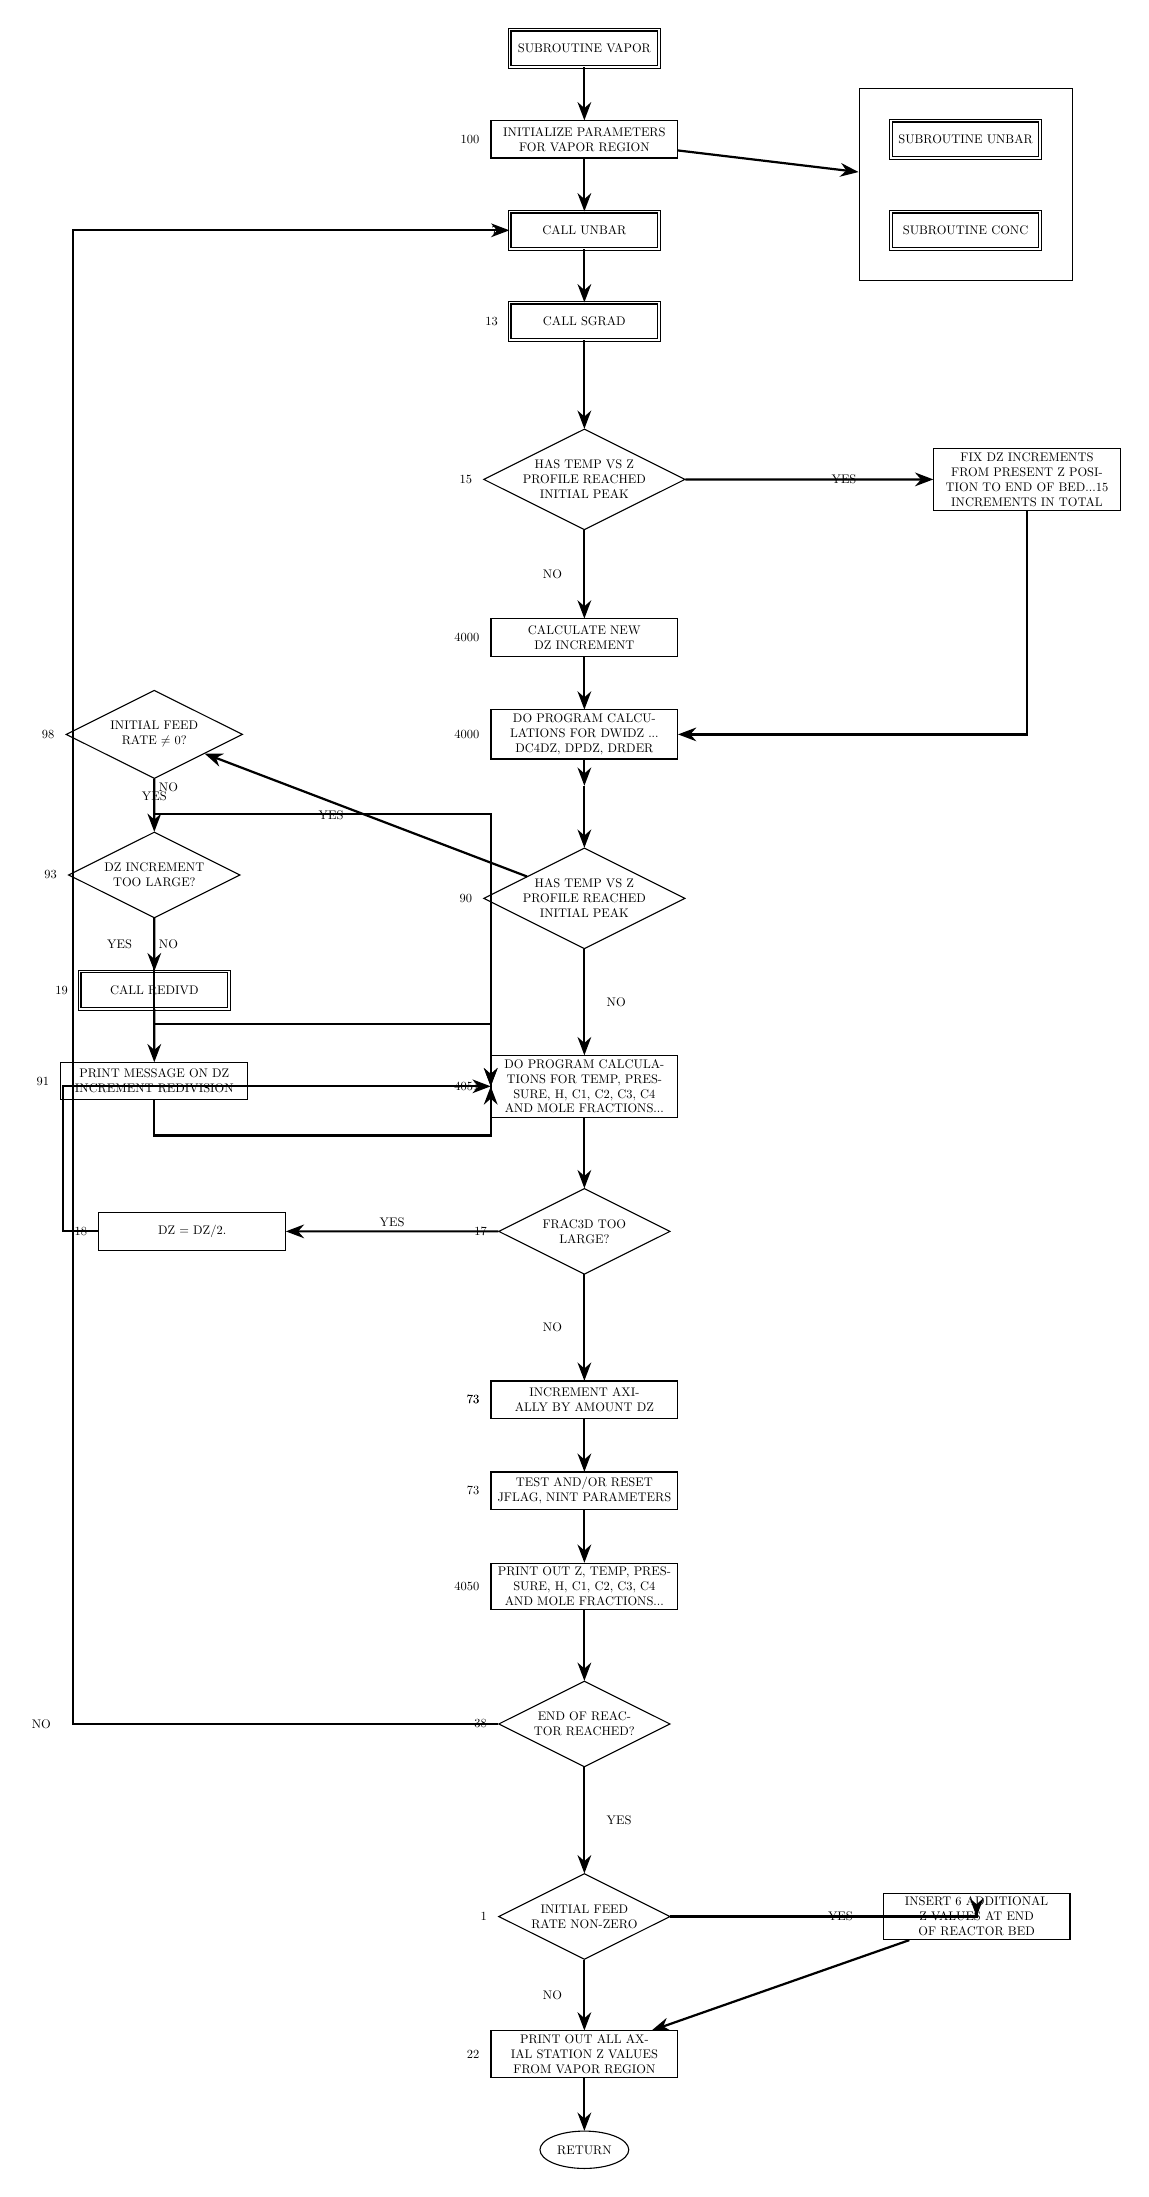
\begin{tikzpicture}[
			scale=0.45, transform shape,
			node distance=1.5cm and 1cm,
			% Define the styles for different blocks
			startstop/.style = {ellipse, draw, text centered, minimum height=3em},
			process/.style = {rectangle, draw, text centered, minimum width=15em, minimum height=3em, align=center, text width=14em},
			subroutine/.style = {rectangle, draw, double, text centered, minimum width=12em, minimum height=3em, align=center, text width=11em},
			decision/.style = {diamond, draw, text centered, minimum width=12em, minimum height=3em, inner sep=0pt, aspect=2, align=center, text width=10em},
			arrow/.style = {draw, -{Stealth[]}, thick}
			]
			
			% --- Nodes from Figure I-3 (Page 82) ---
			\node (vapor) [subroutine] {SUBROUTINE VAPOR};
			
			\node (init) [process, below=of vapor] {INITIALIZE PARAMETERS FOR VAPOR REGION};
			\node (unbar1) [subroutine, below=of init] {CALL UNBAR};
			\node (sgrad) [subroutine, below=of unbar1] {CALL SGRAD};
			\node (dec1) [decision, below=of sgrad, yshift=-1cm] {HAS TEMP VS Z PROFILE REACHED INITIAL PEAK};
			
			\node (fix_dz) [process, right=of dec1, xshift=6cm] {FIX DZ INCREMENTS FROM PRESENT Z POSITION TO END OF BED...15 INCREMENTS IN TOTAL};
			\node (calc_new_dz) [process, below=of dec1, yshift=-1cm] {CALCULATE NEW DZ INCREMENT};
			
			\node (do_calc1) [process, below=of calc_new_dz] {DO PROGRAM CALCULATIONS FOR DWIDZ ... DC4DZ, DPDZ, DRDER};
			% This coordinate is for the loop-back from Fig I-4
			\coordinate (loop_target) at ($(do_calc1.south) + (0,-0.75cm)$);
			\node (dec2) [decision, below=of do_calc1, yshift=-1cm] {HAS TEMP VS Z PROFILE REACHED INITIAL PEAK};
			
			% --- START FIX: MOVED THIS BLOCK BACK TO THE LEFT ---
			\node (dec3) [decision, left=of do_calc1, xshift=-6cm] {INITIAL FEED RATE $\neq$ 0?};
			\node (dec4) [decision, below=of dec3] {DZ INCREMENT TOO LARGE?};
			\node (redivd) [subroutine, below=of dec4] {CALL REDIVD};
			\node (print_rediv) [process, below=of redivd] {PRINT MESSAGE ON DZ INCREMENT REDIVISION};
			% --- END FIX ---
			
			% Side subroutines for init
			\node (unbar2) [subroutine, right=of init, xshift=5cm] {SUBROUTINE UNBAR};
			\node (conc) [subroutine, below=of unbar2, node distance=1cm] {SUBROUTINE CONC};
			\node[draw, inner sep=0.4cm, fit=(unbar2) (conc)] (init_subs) {};
			
			
			% --- Nodes from Figure I-4 (Page 83) ---
			\node (do_calc2) [process, below=of dec2, yshift=-1.5cm] {DO PROGRAM CALCULATIONS FOR TEMP, PRESSURE, H, C1, C2, C3, C4 AND MOLE FRACTIONS...};
			\node (dec5) [decision, below=of do_calc2, yshift=-0.5cm] {FRAC3D TOO LARGE?};
			\node (half_dz) [process, left=of dec5, xshift=-5cm] {DZ = DZ/2.};
			
			\node (inc_dz) [process, below=of dec5, yshift=-1.5cm] {INCREMENT AXIALLY BY AMOUNT DZ};
			\node (test_flags) [process, below=of inc_dz] {TEST AND/OR RESET JFLAG, NINT PARAMETERS};
			\node (print_main) [process, below=of test_flags] {PRINT OUT Z, TEMP, PRESSURE, H, C1, C2, C3, C4 AND MOLE FRACTIONS...};
			\node (dec6) [decision, below=of print_main, yshift=-0.5cm] {END OF REACTOR REACHED?};
			
			\node (dec7) [decision, below=of dec6, yshift=-1.5cm] {INITIAL FEED RATE NON-ZERO};
			\node (insert_z) [process, right=of dec7, xshift=5cm] {INSERT 6 ADDITIONAL Z VALUES AT END OF REACTOR BED};
			\node (print_z) [process, below=of dec7, yshift=-0.5cm] {PRINT OUT ALL AXIAL STATION Z VALUES FROM VAPOR REGION};
			\node (ret) [startstop, below=of print_z] {RETURN};
			
			% --- Draw Arrows ---
			% Fig I-3 flow
			\path [arrow] (vapor) -- (init);
			\path [arrow] (init) -- (init_subs);
			\path [arrow] (init) -- (unbar1);
			\path [arrow] (unbar1) -- (sgrad);
			\path [arrow] (sgrad) -- (dec1);
			
			\path [arrow] (dec1) -- node[right, xshift=5mm] {YES} (fix_dz);
			\path [arrow] (dec1) -- node[left, xshift=-5mm] {NO} (calc_new_dz);
			
			\draw [arrow] (fix_dz.south) |- (do_calc1.east);
			\path [arrow] (calc_new_dz) -- (do_calc1);
			\path [arrow] (do_calc1) -- (loop_target);
			\path [arrow] (loop_target) -- (dec2);
			
			% --- START FIX: Corrected arrow path and label position ---
			\path [arrow] (dec2) -- node[left, xshift=-5mm] {YES} (dec3);
			\path [arrow] (dec3) -- node[above] {YES} (dec4);
			\path [arrow] (dec4) -- node[left, xshift=-5mm] {YES} (redivd);
			% --- END FIX ---
			
			\path [arrow] (redivd) -- (print_rediv);
			
			% Fig I-4 flow
			% --- START FIX: Corrected paths from left-hand branch ---
			\path [arrow] (dec2) -- node[right, xshift=5mm] {NO} (do_calc2);
			\draw [arrow] (dec3.south) -- node[right, near start] {NO} ++(0,-1) -| (do_calc2.west);
			\draw [arrow] (dec4.south) -- node[right, near start] {NO} ++(0,-3) -| (do_calc2.west);
			\draw [arrow] (print_rediv.south) -- ++(0,-1) -| (do_calc2.west);
			% --- END FIX ---
			
			\path [arrow] (do_calc2) -- (dec5);
			\path [arrow] (dec5) -- node[left, xshift=-5mm] {NO} (inc_dz);
			\node[left, xshift=-2mm] at (inc_dz.west) {73};
			\path [arrow] (dec5) -- node[above] {YES} (half_dz);
			\draw [arrow] (half_dz.west) -- ++(-1,0) |- (do_calc2.west);
			
			\path [arrow] (inc_dz) -- (test_flags);
			\path [arrow] (test_flags) -- (print_main);
			\path [arrow] (print_main) -- (dec6);
			
			% Loop back from Fig I-4 to Fig I-3
			\draw [arrow] (dec6.west) -- ++(-12,0) node[left, xshift=-5mm] {NO} |- (unbar1);
			
			% Bottom of Fig I-4
			\path [arrow] (dec6) -- node[right, xshift=5mm] {YES} (dec7);
			\path [arrow] (dec7) -| node[right, pos=0.25] {YES} (insert_z);
			\path [arrow] (dec7) -- node[left, xshift=-5mm] {NO} (print_z);
			\path [arrow] (insert_z) -- (print_z);
			\path [arrow] (print_z) -- (ret);
			
			% --- Add Statement Numbers ---
			\node[left, xshift=-2mm] at (init.west) {100};
			\node[left, xshift=-2mm] at (unbar1.west) {7};
			\node[left, xshift=-2mm] at (sgrad.west) {13};
			\node[left, xshift=-2mm] at (dec1.west) {15};
			\node[left, xshift=-2mm] at (calc_new_dz.west) {4000};
			\node[left, xshift=-2mm] at (do_calc1.west) {4000};
			\node[left, xshift=-2mm] at (dec2.west) {90};
			
			% --- FIX: Moved statement numbers back to the left ---
			\node[left, xshift=-2mm] at (dec3.west) {98};
			\node[left, xshift=-2mm] at (dec4.west) {93};
			\node[left, xshift=-2mm] at (redivd.west) {19};
			\node[left, xshift=-2mm] at (print_rediv.west) {91};
			% --- END FIX ---
			
			\node[left, xshift=-2mm] at (do_calc2.west) {4051};
			\node[left, xshift=-2mm] at (dec5.west) {17};
			\node[left, xshift=-2mm] at (half_dz.west) {18};
			\node[left, xshift=-2mm] at (inc_dz.west) {73};
			\node[left, xshift=-2mm] at (test_flags.west) {73};
			\node[left, xshift=-2mm] at (print_main.west) {4050};
			\node[left, xshift=-2mm] at (dec6.west) {38};
			\node[left, xshift=-2mm] at (dec7.west) {1};
			\node[left, xshift=-2mm] at (print_z.west) {22};
			
		\end{tikzpicture}
		\caption{Figure I-3 \& I-4: SUBROUTINE VAPOR Flow Diagram (Combined)}
		\label{fig:I-3-4}
	\end{figure}
	% --- End of TikZ Diagram ---
	
	\section*{Appendix II: Listing of Computer Programs}
	\addcontentsline{toc}{section}{Appendix II: Listing of Computer Programs}
	
	\subsection*{One-Dimensional Steady-State Model}
	
	\begin{lstlisting}[language=Fortran, caption=MAIN Program Listing, label=list:main_1d]
C **********************************************************************
C * *
C * DESCRIPTION OF INPUT DATA PUNCH CARDS FOLLOWS...                   *
C * *
C **********************************************************************
C
C CARD 1      COL'S 1-3   CONTAIN NCASE   (I3)    (ONLY ONE CARD 1 PER RUN)
C
C (CARDS 2 THRU 16 SHOULD BE REPEATED FOR EACH DATA CASE)
C
C CARD 2      COL'S 1-80  TITLE CARD (14A6) ANY ALPHANUMERIC INFORMATION DESIRED
C
C CARD 3      COL'S 1-2   CONTAIN OPTION  (I2)
C             COL'S 3-4   CONTAIN PRINT   (I2)
C             COL'S 5-7   CONTAIN NOFZ    (I3)
C
C CARD 4      COL'S 1-10  CONTAIN ZO      (E10.5)
C             COL'S 11-20 CONTAIN GO      (E10.5)
C             COL'S 21-30 CONTAIN FC      (E10.5)
C             COL'S 31-40 CONTAIN ALPHA3  (E10.5)
C             COL'S 41-50 CONTAIN HF      (E10.5)
C             COL'S 51-60 CONTAIN R       (E10.5)
C             COL'S 61-70 CONTAIN WM4     (E10.5)
C             COL'S 71-80 CONTAIN WM3     (E10.5)
C
C CARD 5      COL'S 1-10  CONTAIN WM2     (E10.5)
C             COL'S 11-20 CONTAIN WM1     (E10.5)
C             COL'S 21-30 CONTAIN ALPHA1  (E10.5)
C             COL'S 31-40 CONTAIN ALPHA2  (E10.5)
C             COL'S 41-50 CONTAIN AGM     (E10.5)
C             COL'S 51-60 CONTAIN BGM     (E10.5)
C             COL'S 61-70 CONTAIN KP      (E10.5)
C             COL'S 71-80 CONTAIN CGM     (E10.5)
C
C CARD 6      COL'S 1-10  CONTAIN TF      (E10.5)
C             COL'S 11-20 CONTAIN CFL     (E10.5)
C             COL'S 21-30 CONTAIN ENMX1   (E10.5)
C             COL'S 31-40 CONTAIN ENMX2   (E10.5)
C             COL'S 41-50 CONTAIN ENMX3   (E10.5)
C             COL'S 51-60 CONTAIN DIF3    (E10.5)
C             COL'S 61-70 CONTAIN DIF4    (E10.5)
C             COL'S 71-80 CONTAIN PRES    (E10.5)
C
C CARD 7      COL'S 1-10  CONTAIN ZEND    (E10.5)
C             COL'S 11-20 CONTAIN EN1     (E10.5)
C             COL'S 21-30 CONTAIN EN2     (E10.5)
C             COL'S 31-40 CONTAIN EN3     (E10.5)
C
C (THE TABLE FOR CATALYST PARTICLE RADIUS VS
C  AXIAL DISTANCE ALONG REACTOR BED FOLLOWS)
C
C CARD 8      COL'S 1-8   CONTAIN THE NUMBER 0.0      (E8.4)
C             COL'S 9-16  CONTAIN THE NUMBER 1.0      (E8.4)
C             COL'S 17-24 CONTAIN NOFZ (FLOATING POINT) (E8.4)
C             COL'S 25-32 CONTAIN THE NUMBER 0.0      (E8.4)
C
C CARDS 9A,9B...  CONTAIN THE AXIAL STATION Z VALUES  (10E8.4)
C             Z(1),Z(2),....Z(NOFZ)
C             10 PER CARD, COL'S 1-80
C
C CARDS 10A,10B... CONTAIN THE CATALYST PARTICLE RADII (10E8.4)
C             A(1),A(2),....A(NOFZ)
C             10 PER CARD, COL'S 1-80
C
C (THE TABLE FOR CATALYST PARTICLE SURFACE AREA
C  VS AXIAL DISTANCE ALONG REACTOR BED FOLLOWS)
C
C CARD 11     THIS CARD IS IDENTICAL TO CARD 8
C
C CARDS 12A,12B... THESE CARDS (OR SINGLE CARD) ARE IDENTICAL TO CARDS 9A,9B...
C
C CARDS 13A,13B... CONTAIN THE CATALYST PARTICLE SURFACE AREAS (10E8.4)
C             AP(1),AP(2),...AP(NOFZ)
C             10 PER CARD, COL'S 1-80
C
C (THE TABLE FOR INTERPARTICLE VOID FRACTION VS
C  AXIAL DISTANCE ALONG REACTOR BED FOLLOWS)
C
C CARD 14     THIS CARD IS IDENTICAL TO CARD 8
C
C CARDS 15A,15B... THESE CARDS (OR SINGLE CARD) ARE IDENTICAL TO CARDS 9A,9B...
C
C CARDS 16A,16B... CONTAIN THE INTERPARTICLE VOID FRACTIONS (10E8.4)
C             DELA(1),DELA(2),....DELA(NOFZ)
C             10 PER CARD, COL'S 1-80
C
REAL KP,K 															   0
INTEGER OPTION,PRINT												  10
COMMON /FTZ/TBLVP(70),TBLH4(42),TBLH3(42),SHTBL1(34),SHTBL2(34), 	  20
1        SHTBL3(34),SHTBL4(34),ZTBLD(46),ZTBLAP(46),ZTBLA(46) 		  30
COMMON /CO/HL,HV,FC,TF,CFL,CGM,ENMX1,AGM,DIF3,DIF4,KP,PRES,G0,		  40
1        WM4,WM3,WM2,WM1,ALPHA3,R,TVAP,ZEND,BGM,HF,DZ,ALPHA1,ALPHA2	  50
2        ,ENMX2,ENMX3,EN1,EN2,EN3,H,RAT,MI 							  60
COMMON /VAR/DERIV(250),DHDZ(250),Z(250)								  70
COMMON /TOLL/ALIM,OPTION,C1,C2,C3,C4,CAV,G,TEMP,AP,WMAV,Z0,			  80
COMMON /MUVST/VISVST(30)											  90
COMMON /FLAGS/MFLAG,KFLAG,PRINT 									 100
COMMON /IFCE00/IFC,GATZ0											 110
COMMON /LIZTBL/DHVST(18),DHLVST(18)									 120
COMMON /DAVTBL/VPTBL(44)											 130
DIMENSION  TITLE(14) 												 140
READ (5,700) NCASE 													 150
700 FORMAT (I3)															 160
KOUNT=1																 170
705 READ (5,608) TITLE 													 180
608 FORMAT (14A6)														 190
WRITE (6,609) TITLE													 200
609 FORMAT (1H1,14A6//)													 210
IFC=1																 220
READ (5,809) OPTION,PRINT,NOFZ										 230
809 FORMAT (2I2,I3)														 240
READ (5,800) Z0,G0,FC,ALPHA3,HF,R,WM4,WM3,WM2,WM1,ALPHA1,ALPHA2,	 250
X      AGM,BGM,KP,CGM,TF,CFL,ENMX1,ENMX2,ENMX3,DIF3,DIF4,PRES,ZEND,   260
X      EN1,EN2,EN3,													 270
800 FORMAT (8E10.5)														 280
NZTBL = 2*NOFZ+4													 290
NOFZ4 = NOFZ+4														 300
NOFZ5 = NOFZ4+1 													 310
CALL UNBAR (VPTBL(1),1,PRES,0.,TVAP,KK)								 320
CALL UNBAR (DHVST(1),1,TVAP,0.,DELHV,KK)							 330
CALL UNBAR (DHLVST(1),1,TVAP,0.,DELHL,KK)							 340
HL=(TVAP-TF)*CFL													 350
HV=HL+DELHV-DELHL													 360
GATZ0=G0+FC*Z0														 370
IF(FC.GT.0.)GO TO 837												 380
IFC=0																 390
637 WRITE (6,600)														 400
600 FORMAT (52X,16H INPUT CONSTANTS/7X,102H HF      HL        HV  	     410
X       TF      TVAP    CFL     PRESSURE    KP    FC                 420
X       G0) 															 430
WRITE (6,601) HF,HL,HV,TF,TVAP,CFL,PRES,KP,FC,G0					 440
601 FORMAT (3X,10E11.6//)												 450
WRITE (6,602)														 460
602 FORMAT (7X,103H  R    ALPHA3   CGM   DIF3    DIF4 					 470
X        WM4     WM3   
X   WM2     WM1   ZEND)							 480
WRITE (6,601) R,ALPHA3,CGM,DIF3,DIF4,WM4,WM3,WM1,WM1,ZEND			 490
WRITE (6,603)														 500
603	FORMAT (6X,113H  AGM   BGM   ALPHA1    ALPHA2   N1 					 510
X   N2    N3   ENMX1   ENMX2   ENMX3     )							 520
WRITE (6,601) AGM,BGM,ALPHA1,ALPHA2,EN1,EN2,EN3,ENMX1,ENMX2,ENMX3    530
WRITE (6,617) Z0													 540
617 FORMAT (// 8X,'Z0' / 3X,E11.6)										 550
READ (5,20) (ZTBLA(I),I=1,4)										 560
20 FORMAT (4E8.4)														 570
READ (5,21) (ZTBLA(I),I=5,NOFZ4)    								 580
21 FORMAT (10E8.4) 													 590
READ (5,21) (ZTBLA(I),I=NOFZ5,NZTBL)								 600
READ (5,20) (ZTBLAP(I),I=1,4)										 610
READ (5,21) (ZTBLAP(I),I=5,NOFZ4)									 620
READ (5,21) (ZTBLAP(I),I=NOFZ5,NZTBL)								 630
READ (5,20) (ZTBLD(I),I=1,4)										 640
READ (5,21) (ZTBLD(I),I=5,NOFZ4)									 650
READ (5,21) (ZTBLD(I),I=NOFZ5,NZTBL)								 660
WRITE (6,604)														 670
604	FORMAT (///55X,13H Z VS A TABLE)									 680
WRITE (6,22) (ZTBLA(I),I=1,4)										 690
22 FORMAT (40X,4E13.5)												     700
WRITE (6,23) (ZTBLA(I),I=5,NOFZ4)									 710
23 FORMAT (1X,10E13.5)													 720
WRITE (6,25)														 730
25 FORMAT ( / ) 														 740
WRITE (6,23) (ZTBLA(I),I=NOFZ5,NZTBL)								 750
WRITE (6,24) 														 760
24 FORMAT ( // )														 770
WRITE (6,606)														 780
606 FORMAT (54X,14H Z VS AP TABLE)										 790
WRITE (6,22) (ZTBLAP(I),I=1,4)										 800
WRITE (6,23) (ZTBLAP(I),I=5,NOFZ4)									 810
WRITE (6,25)														 820
WRITE (6,23) (ZTBLAP(I),I=NOFZ5,NZTBL)								 830
WRITE (6,24) 														 840
WRITE (6,607)														 850
607 FORMAT (54X,14H Z VS DELTA TABLE)									 860
WRITE (6,22) (ZTBLD(I),I=1,4)										 870
WRITE (6,23) (ZTBLD(I),I=5,NOFZ4)									 880
WRITE (6,25)														 890
WRITE (6,23) (ZTBLD(I),I=NOFZ5,NZTBL)								 900
WRITE (6,613) 														 910
613 FORMAT (18X, ******************************** ENTERING LIQUID        920
X REGION     ********************************) 						 930
MFLAG=0																 940
DZ=0.0																 950
Z(1)=0.0															 960
H=HF																 970
II=2																 980
850 Z(II)=Z(II-1)+DZ 													 990
TEMP=TF+(H-HF)/CFL													1000
CALL UNBAR (TBLVP(I),1,TEMP,0.,VP,KK)								1010
CN2H4=(VP*WM4)/(R*TEMP)												1020
CALL UNBAR (TBLH4(I),1,TEMP,0.,H4,KK)								1030
CALL UNBAR (ZTBLAP(I),1,Z(II),0.,AP,KK)								1040
CALL UNBAR (ZTBLA(I),1,Z(II),0.,A,KK)								1050
CALL PARAM(TEMP,Z(II),1,CN2H4,H4,0,G,GMMA,K,DPA,BETA)				1060
CALL SLOPE (CN2H4,GMMA,K,BETA,EN1,DERIV(II),DPA,A,DIF4)			    1070
IF(H-HL)777,776,777													1080
776 IF(MI.GT.20)DERIV(II)=DERIV(II-1)									1090
777 DHDZ(II)=-(H4*DPA*AP*DERIV(II)+FC*(H-HF))/G							1100
DZ=-H4/(ENMX1*DHDZ(II))												1110
WRITE(6,820)														1120
820 FORMAT (/39X,48H  Z    TEMP    H DHDZ)								1130
WRITE(6,860) Z(II),TEMP,H,DHDZ(II)									1140
860 FORMAT (/30X,4E15.6)												1150
IF(H-HL) 874,1020,874												1160
874 H=H+DHDZ(II)*DZ														1170
IF(H-HL) 875,1020,1000												1180
875 II=II+1																1190
GO TO 850															1200
C		BACKSTEP TO L-L-V-BOUNDARY 											
1000 DZ=(HL-H)/DHDZ(II)+DZ												1210
H=HL																1220
II=II+1																1230
GO TO 850															1240
1020 IF(OPTION.EQ.2) CALL LQV2(H,Z(II),DERIV(II),II,DHDZ(II),TEMP,CN2H4) 1250
IF(OPTION.EQ.2) GO 													1260
TO 1021
CALL LQVP(H,Z(II),DERIV(II),II,DHDZ(II),TEMP)						1270
C		START VAPOR REGION
1021 DZ=-H4/(ENMX2*DHDZ(II))												1280
CALL VAPOR(TEMP,Z(II),II,DHDZ(II),DERIV(II),H)						1290
KOUNT=KOUNT+1														1300
IF(KOUNT.LE.NCASE) GO TO 705 										1310
WRITE(6,102)														1320
102 FORMAT (////41X,36H ***** OPERATIONS COMPLETE *****)				1330
STOP																1340
END																	1350
	\end{lstlisting}
	
	
	
	
	
	
	
	\include{app-NASA9.tex}
	
	
	
	
	
	
	
	
	
	
	
	
	
	
	
	
	
	
	
	
	
	
	
	
	
	
\end{document}